\documentclass[../main.tex]{subfiles}


\title{Calculus}
\author{}
\date{}

\begin{document}

\maketitle
\tableofcontents

\newpage

\section{Derivatives and Integrals}

\subsection{Derivatives}

A function measures some quantity over time.
Imagine a vacuum collecting particles.
If \( f \) is the measure of the number of particles in the tank at time \( t \),
then \( f \) is the accumulation of particles.
And \( f' \) is just the rate of accumulation at a given time.
And likewise, if \( g \) measures the rate of particles going in,
then \( \int g \) is the total amount of particles collected.

Velocity is the first derivative of position.
Acceleration is the second derivative.
Velocity is the accumulation of acceleration, or its integral.
Position is the accumulation of velocity, or its integral.

\begin{tikzpicture}[x=0.75pt,y=0.75pt,yscale=-1,xscale=1]
%uncomment if require: \path (0,300); %set diagram left start at 0, and has height of 300

%Shape: Axis 2D [id:dp791486377406529] 
\draw  (50,241.7) -- (314.5,241.7)(76.45,41) -- (76.45,264) (307.5,236.7) -- (314.5,241.7) -- (307.5,246.7) (71.45,48) -- (76.45,41) -- (81.45,48) (115.45,236.7) -- (115.45,246.7)(154.45,236.7) -- (154.45,246.7)(193.45,236.7) -- (193.45,246.7)(232.45,236.7) -- (232.45,246.7)(271.45,236.7) -- (271.45,246.7)(71.45,202.7) -- (81.45,202.7)(71.45,163.7) -- (81.45,163.7)(71.45,124.7) -- (81.45,124.7)(71.45,85.7) -- (81.45,85.7) ;
\draw   ;
%Curve Lines [id:da6119806462814916] 
\draw    (76.45,241.7) .. controls (112.5,67) and (290.5,90) .. (292.5,82) ;
%Shape: Axis 2D [id:dp1956952642703632] 
\draw  (370,238.7) -- (634.5,238.7)(396.45,38) -- (396.45,261) (627.5,233.7) -- (634.5,238.7) -- (627.5,243.7) (391.45,45) -- (396.45,38) -- (401.45,45) (435.45,233.7) -- (435.45,243.7)(474.45,233.7) -- (474.45,243.7)(513.45,233.7) -- (513.45,243.7)(552.45,233.7) -- (552.45,243.7)(591.45,233.7) -- (591.45,243.7)(391.45,199.7) -- (401.45,199.7)(391.45,160.7) -- (401.45,160.7)(391.45,121.7) -- (401.45,121.7)(391.45,82.7) -- (401.45,82.7) ;
\draw   ;
%Curve Lines [id:da6904688712857534] 
\draw    (396.45,238.7) .. controls (432.5,64) and (610.5,87) .. (612.5,79) ;
%Straight Lines [id:da8868203342962732] 
\draw [color={rgb, 255:red, 255; green, 0; blue, 0 }  ,draw opacity=1 ]   (396.45,238.7) -- (429.5,159) ;
%Straight Lines [id:da6732443966151707] 
\draw [color={rgb, 255:red, 255; green, 0; blue, 0 }  ,draw opacity=1 ]   (429.5,159) -- (494.5,105) ;
%Straight Lines [id:da792722354522738] 
\draw [color={rgb, 255:red, 255; green, 0; blue, 0 }  ,draw opacity=1 ]   (600.5,81) -- (494.5,105) ;
%Straight Lines [id:da7780337638207823] 
\draw [color={rgb, 255:red, 0; green, 42; blue, 255 }  ,draw opacity=1 ]   (429.5,159) -- (493.5,159) ;
%Straight Lines [id:da5469718819271276] 
\draw [color={rgb, 255:red, 0; green, 42; blue, 255 }  ,draw opacity=1 ]   (493.5,159) -- (493.5,107) ;

% Text Node
\draw (42,139.4) node [anchor=north west][inner sep=0.75pt]    {$y$};
% Text Node
\draw (174,263.4) node [anchor=north west][inner sep=0.75pt]    {$x$};
% Text Node
\draw (362,136.4) node [anchor=north west][inner sep=0.75pt]    {$y$};
% Text Node
\draw (494,260.4) node [anchor=north west][inner sep=0.75pt]    {$x$};
% Text Node
\draw (454,167.4) node [anchor=north west][inner sep=0.75pt]  [color={rgb, 255:red, 0; green, 95; blue, 255 }  ,opacity=1 ]  {$dx$};
% Text Node
\draw (504,126.4) node [anchor=north west][inner sep=0.75pt]  [color={rgb, 255:red, 0; green, 24; blue, 255 }  ,opacity=1 ]  {$dy$};
% Text Node
\draw (407,75.4) node [anchor=north west][inner sep=0.75pt]  [color={rgb, 255:red, 255; green, 0; blue, 0 }  ,opacity=1 ]  {$\sqrt{dx^{2} +dy^{2}}$};


\end{tikzpicture}

Since acceleration is the change in velocity,
adding an acceleration vector to the velocity vector gives the resultant velocity vector.

For a single variable function, we only care about the quantity varying in one dimension,
parameterized by a one dimensional input.


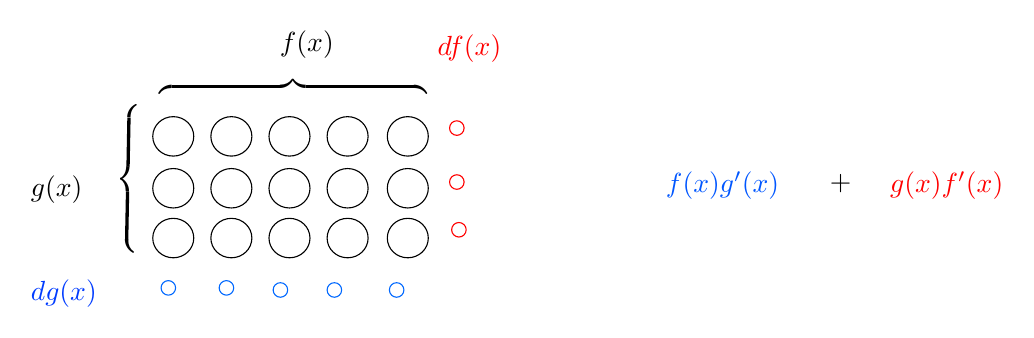
\begin{tikzpicture}[x=0.75pt,y=0.75pt,yscale=-1,xscale=1]
%uncomment if require: \path (0,300); %set diagram left start at 0, and has height of 300

%Shape: Ellipse [id:dp06031973450750061] 
\draw   (164,126.5) .. controls (164,121.25) and (168.42,117) .. (173.88,117) .. controls (179.33,117) and (183.75,121.25) .. (183.75,126.5) .. controls (183.75,131.75) and (179.33,136) .. (173.88,136) .. controls (168.42,136) and (164,131.75) .. (164,126.5) -- cycle ;
%Shape: Ellipse [id:dp8478408655553544] 
\draw   (192,126.5) .. controls (192,121.25) and (196.42,117) .. (201.88,117) .. controls (207.33,117) and (211.75,121.25) .. (211.75,126.5) .. controls (211.75,131.75) and (207.33,136) .. (201.88,136) .. controls (196.42,136) and (192,131.75) .. (192,126.5) -- cycle ;
%Shape: Ellipse [id:dp505421117341947] 
\draw   (220,126.5) .. controls (220,121.25) and (224.42,117) .. (229.88,117) .. controls (235.33,117) and (239.75,121.25) .. (239.75,126.5) .. controls (239.75,131.75) and (235.33,136) .. (229.88,136) .. controls (224.42,136) and (220,131.75) .. (220,126.5) -- cycle ;
%Shape: Ellipse [id:dp007218742660141997] 
\draw   (248,126.5) .. controls (248,121.25) and (252.42,117) .. (257.88,117) .. controls (263.33,117) and (267.75,121.25) .. (267.75,126.5) .. controls (267.75,131.75) and (263.33,136) .. (257.88,136) .. controls (252.42,136) and (248,131.75) .. (248,126.5) -- cycle ;
%Shape: Ellipse [id:dp8702465733669611] 
\draw   (277,126.5) .. controls (277,121.25) and (281.42,117) .. (286.88,117) .. controls (292.33,117) and (296.75,121.25) .. (296.75,126.5) .. controls (296.75,131.75) and (292.33,136) .. (286.88,136) .. controls (281.42,136) and (277,131.75) .. (277,126.5) -- cycle ;
%Shape: Ellipse [id:dp6716570870833466] 
\draw   (164,151.5) .. controls (164,146.25) and (168.42,142) .. (173.88,142) .. controls (179.33,142) and (183.75,146.25) .. (183.75,151.5) .. controls (183.75,156.75) and (179.33,161) .. (173.88,161) .. controls (168.42,161) and (164,156.75) .. (164,151.5) -- cycle ;
%Shape: Ellipse [id:dp1820921953890161] 
\draw   (192,151.5) .. controls (192,146.25) and (196.42,142) .. (201.88,142) .. controls (207.33,142) and (211.75,146.25) .. (211.75,151.5) .. controls (211.75,156.75) and (207.33,161) .. (201.88,161) .. controls (196.42,161) and (192,156.75) .. (192,151.5) -- cycle ;
%Shape: Ellipse [id:dp5866793827026061] 
\draw   (220,151.5) .. controls (220,146.25) and (224.42,142) .. (229.88,142) .. controls (235.33,142) and (239.75,146.25) .. (239.75,151.5) .. controls (239.75,156.75) and (235.33,161) .. (229.88,161) .. controls (224.42,161) and (220,156.75) .. (220,151.5) -- cycle ;
%Shape: Ellipse [id:dp45797332679454195] 
\draw   (248,151.5) .. controls (248,146.25) and (252.42,142) .. (257.88,142) .. controls (263.33,142) and (267.75,146.25) .. (267.75,151.5) .. controls (267.75,156.75) and (263.33,161) .. (257.88,161) .. controls (252.42,161) and (248,156.75) .. (248,151.5) -- cycle ;
%Shape: Ellipse [id:dp24430516488734677] 
\draw   (277,151.5) .. controls (277,146.25) and (281.42,142) .. (286.88,142) .. controls (292.33,142) and (296.75,146.25) .. (296.75,151.5) .. controls (296.75,156.75) and (292.33,161) .. (286.88,161) .. controls (281.42,161) and (277,156.75) .. (277,151.5) -- cycle ;
%Shape: Ellipse [id:dp5662108764983852] 
\draw   (164,175.5) .. controls (164,170.25) and (168.42,166) .. (173.88,166) .. controls (179.33,166) and (183.75,170.25) .. (183.75,175.5) .. controls (183.75,180.75) and (179.33,185) .. (173.88,185) .. controls (168.42,185) and (164,180.75) .. (164,175.5) -- cycle ;
%Shape: Ellipse [id:dp6579543801408282] 
\draw   (192,175.5) .. controls (192,170.25) and (196.42,166) .. (201.88,166) .. controls (207.33,166) and (211.75,170.25) .. (211.75,175.5) .. controls (211.75,180.75) and (207.33,185) .. (201.88,185) .. controls (196.42,185) and (192,180.75) .. (192,175.5) -- cycle ;
%Shape: Ellipse [id:dp17883475704623442] 
\draw   (220,175.5) .. controls (220,170.25) and (224.42,166) .. (229.88,166) .. controls (235.33,166) and (239.75,170.25) .. (239.75,175.5) .. controls (239.75,180.75) and (235.33,185) .. (229.88,185) .. controls (224.42,185) and (220,180.75) .. (220,175.5) -- cycle ;
%Shape: Ellipse [id:dp8959152379599131] 
\draw   (248,175.5) .. controls (248,170.25) and (252.42,166) .. (257.88,166) .. controls (263.33,166) and (267.75,170.25) .. (267.75,175.5) .. controls (267.75,180.75) and (263.33,185) .. (257.88,185) .. controls (252.42,185) and (248,180.75) .. (248,175.5) -- cycle ;
%Shape: Ellipse [id:dp8976107913184502] 
\draw   (277,175.5) .. controls (277,170.25) and (281.42,166) .. (286.88,166) .. controls (292.33,166) and (296.75,170.25) .. (296.75,175.5) .. controls (296.75,180.75) and (292.33,185) .. (286.88,185) .. controls (281.42,185) and (277,180.75) .. (277,175.5) -- cycle ;
%Shape: Circle [id:dp01856382719091243] 
\draw  [color={rgb, 255:red, 255; green, 0; blue, 0 }  ,draw opacity=1 ] (307,122.5) .. controls (307,120.57) and (308.57,119) .. (310.5,119) .. controls (312.43,119) and (314,120.57) .. (314,122.5) .. controls (314,124.43) and (312.43,126) .. (310.5,126) .. controls (308.57,126) and (307,124.43) .. (307,122.5) -- cycle ;
%Shape: Circle [id:dp4403664682847295] 
\draw  [color={rgb, 255:red, 0; green, 104; blue, 255 }  ,draw opacity=1 ] (168,199.5) .. controls (168,197.57) and (169.57,196) .. (171.5,196) .. controls (173.43,196) and (175,197.57) .. (175,199.5) .. controls (175,201.43) and (173.43,203) .. (171.5,203) .. controls (169.57,203) and (168,201.43) .. (168,199.5) -- cycle ;
%Shape: Circle [id:dp07179694909069678] 
\draw  [color={rgb, 255:red, 0; green, 104; blue, 255 }  ,draw opacity=1 ] (196,199.5) .. controls (196,197.57) and (197.57,196) .. (199.5,196) .. controls (201.43,196) and (203,197.57) .. (203,199.5) .. controls (203,201.43) and (201.43,203) .. (199.5,203) .. controls (197.57,203) and (196,201.43) .. (196,199.5) -- cycle ;
%Shape: Circle [id:dp1451673451815234] 
\draw  [color={rgb, 255:red, 0; green, 104; blue, 255 }  ,draw opacity=1 ] (222,200.5) .. controls (222,198.57) and (223.57,197) .. (225.5,197) .. controls (227.43,197) and (229,198.57) .. (229,200.5) .. controls (229,202.43) and (227.43,204) .. (225.5,204) .. controls (223.57,204) and (222,202.43) .. (222,200.5) -- cycle ;
%Shape: Circle [id:dp9161876920152885] 
\draw  [color={rgb, 255:red, 0; green, 104; blue, 255 }  ,draw opacity=1 ] (248,200.5) .. controls (248,198.57) and (249.57,197) .. (251.5,197) .. controls (253.43,197) and (255,198.57) .. (255,200.5) .. controls (255,202.43) and (253.43,204) .. (251.5,204) .. controls (249.57,204) and (248,202.43) .. (248,200.5) -- cycle ;
%Shape: Circle [id:dp7144565199430419] 
\draw  [color={rgb, 255:red, 0; green, 104; blue, 255 }  ,draw opacity=1 ] (278,200.5) .. controls (278,198.57) and (279.57,197) .. (281.5,197) .. controls (283.43,197) and (285,198.57) .. (285,200.5) .. controls (285,202.43) and (283.43,204) .. (281.5,204) .. controls (279.57,204) and (278,202.43) .. (278,200.5) -- cycle ;
%Shape: Circle [id:dp8377649456481785] 
\draw  [color={rgb, 255:red, 255; green, 0; blue, 0 }  ,draw opacity=1 ] (307,148.5) .. controls (307,146.57) and (308.57,145) .. (310.5,145) .. controls (312.43,145) and (314,146.57) .. (314,148.5) .. controls (314,150.43) and (312.43,152) .. (310.5,152) .. controls (308.57,152) and (307,150.43) .. (307,148.5) -- cycle ;
%Shape: Circle [id:dp940388133671272] 
\draw  [color={rgb, 255:red, 255; green, 0; blue, 0 }  ,draw opacity=1 ] (308,171.5) .. controls (308,169.57) and (309.57,168) .. (311.5,168) .. controls (313.43,168) and (315,169.57) .. (315,171.5) .. controls (315,173.43) and (313.43,175) .. (311.5,175) .. controls (309.57,175) and (308,173.43) .. (308,171.5) -- cycle ;

% Text Node
\draw (224,74.4) node [anchor=north west][inner sep=0.75pt]    {$f( x)$};
% Text Node
\draw (166,96.4) node [anchor=north west][inner sep=0.75pt]    {$\overbrace{\ \ \ \ \ \ \ \ \ \ \ \ \ \ \ \ \ \ \ \ \ \ \ \ \ \ \ \ \ }$};
% Text Node
\draw (145.21,183.74) node [anchor=north west][inner sep=0.75pt]  [rotate=-271.09]  {$\overbrace{\ \ \ \ \ \ \ \ \ \ \ \ \ \ \ \ }$};
% Text Node
\draw (104,144.4) node [anchor=north west][inner sep=0.75pt]    {$g( x)$};
% Text Node
\draw (300,76.4) node [anchor=north west][inner sep=0.75pt]  [color={rgb, 255:red, 255; green, 0; blue, 0 }  ,opacity=1 ]  {$df( x)$};
% Text Node
\draw (104,194.4) node [anchor=north west][inner sep=0.75pt]  [color={rgb, 255:red, 0; green, 59; blue, 255 }  ,opacity=1 ]  {$dg( x)$};
% Text Node
\draw (410,142.4) node [anchor=north west][inner sep=0.75pt]  [color={rgb, 255:red, 0; green, 86; blue, 255 }  ,opacity=1 ]  {$f( x) g'( x)$};
% Text Node
\draw (489,143.4) node [anchor=north west][inner sep=0.75pt]    {$+$};
% Text Node
\draw (518,142.4) node [anchor=north west][inner sep=0.75pt]  [color={rgb, 255:red, 255; green, 0; blue, 0 }  ,opacity=1 ]  {$g( x) f'( x)$};


\end{tikzpicture}

Graphically, the derivative of a function is just the vertical velocity of the "ball"
and the second derivative is the vertical acceleration.


\subsection{Finding the Derivative}


How do we find the derivative at a point, from a graph?
What we want is the velocity or the change in distance per change in time,
but this has no meaning at a single moment.
What we do is find the limit of the changes.

\begin{tikzpicture}[x=0.75pt,y=0.75pt,yscale=-1,xscale=1]
%uncomment if require: \path (0,300); %set diagram left start at 0, and has height of 300

%Shape: Axis 2D [id:dp3419332376667883] 
\draw  (41,249) -- (334.5,249)(78.73,15) -- (78.73,274) (327.5,244) -- (334.5,249) -- (327.5,254) (73.73,22) -- (78.73,15) -- (83.73,22) (127.73,244) -- (127.73,254)(176.73,244) -- (176.73,254)(225.73,244) -- (225.73,254)(274.73,244) -- (274.73,254)(73.73,200) -- (83.73,200)(73.73,151) -- (83.73,151)(73.73,102) -- (83.73,102)(73.73,53) -- (83.73,53) ;
\draw   ;
%Shape: Circle [id:dp15714841919076528] 
\draw   (278,132.75) .. controls (278,129.57) and (280.57,127) .. (283.75,127) .. controls (286.93,127) and (289.5,129.57) .. (289.5,132.75) .. controls (289.5,135.93) and (286.93,138.5) .. (283.75,138.5) .. controls (280.57,138.5) and (278,135.93) .. (278,132.75) -- cycle ;
%Curve Lines [id:da48902714333738084] 
\draw    (79,183) .. controls (88.79,175.66) and (92.03,119.89) .. (120.27,166.95) .. controls (148.5,214) and (187.02,172.39) .. (223.5,199) .. controls (259.98,225.61) and (248.5,129) .. (278,132.75) ;
%Straight Lines [id:da8141145633432557] 
\draw [color={rgb, 255:red, 255; green, 0; blue, 0 }  ,draw opacity=1 ]   (283,115) -- (283,74) ;
\draw [shift={(283,72)}, rotate = 450] [color={rgb, 255:red, 255; green, 0; blue, 0 }  ,draw opacity=1 ][line width=0.75]    (10.93,-3.29) .. controls (6.95,-1.4) and (3.31,-0.3) .. (0,0) .. controls (3.31,0.3) and (6.95,1.4) .. (10.93,3.29)   ;
%Straight Lines [id:da3154003786291655] 
\draw [color={rgb, 255:red, 255; green, 0; blue, 0 }  ,draw opacity=1 ]   (282.75,148.5) -- (282.75,187) ;
\draw [shift={(282.75,189)}, rotate = 270] [color={rgb, 255:red, 255; green, 0; blue, 0 }  ,draw opacity=1 ][line width=0.75]    (10.93,-3.29) .. controls (6.95,-1.4) and (3.31,-0.3) .. (0,0) .. controls (3.31,0.3) and (6.95,1.4) .. (10.93,3.29)   ;
%Straight Lines [id:da19276906577043762] 
\draw  [dash pattern={on 0.84pt off 2.51pt}]  (283.75,138.5) -- (283.75,257) ;
%Straight Lines [id:da9895246969397727] 
\draw [color={rgb, 255:red, 0; green, 42; blue, 255 }  ,draw opacity=1 ]   (248,272) -- (279.5,272) ;
\draw [shift={(281.5,272)}, rotate = 180] [color={rgb, 255:red, 0; green, 42; blue, 255 }  ,draw opacity=1 ][line width=0.75]    (10.93,-3.29) .. controls (6.95,-1.4) and (3.31,-0.3) .. (0,0) .. controls (3.31,0.3) and (6.95,1.4) .. (10.93,3.29)   ;
%Shape: Axis 2D [id:dp074444405148542] 
\draw  (338,248) -- (631.5,248)(375.73,14) -- (375.73,273) (624.5,243) -- (631.5,248) -- (624.5,253) (370.73,21) -- (375.73,14) -- (380.73,21) (424.73,243) -- (424.73,253)(473.73,243) -- (473.73,253)(522.73,243) -- (522.73,253)(571.73,243) -- (571.73,253)(370.73,199) -- (380.73,199)(370.73,150) -- (380.73,150)(370.73,101) -- (380.73,101)(370.73,52) -- (380.73,52) ;
\draw   ;
%Shape: Circle [id:dp6593224815387302] 
\draw   (575,131.75) .. controls (575,128.57) and (577.57,126) .. (580.75,126) .. controls (583.93,126) and (586.5,128.57) .. (586.5,131.75) .. controls (586.5,134.93) and (583.93,137.5) .. (580.75,137.5) .. controls (577.57,137.5) and (575,134.93) .. (575,131.75) -- cycle ;
%Curve Lines [id:da4000391883296601] 
\draw    (376,182) .. controls (385.79,174.66) and (412.27,121.95) .. (440.5,169) .. controls (468.73,216.05) and (458.02,173.39) .. (494.5,200) .. controls (530.98,226.61) and (540.5,199) .. (575,131.75) ;
%Straight Lines [id:da6430080624749632] 
\draw [color={rgb, 255:red, 255; green, 0; blue, 0 }  ,draw opacity=1 ]   (580,114) -- (580,73) ;
\draw [shift={(580,71)}, rotate = 450] [color={rgb, 255:red, 255; green, 0; blue, 0 }  ,draw opacity=1 ][line width=0.75]    (10.93,-3.29) .. controls (6.95,-1.4) and (3.31,-0.3) .. (0,0) .. controls (3.31,0.3) and (6.95,1.4) .. (10.93,3.29)   ;
%Straight Lines [id:da3118969368266129] 
\draw [color={rgb, 255:red, 255; green, 0; blue, 0 }  ,draw opacity=1 ]   (579.75,147.5) -- (579.75,186) ;
\draw [shift={(579.75,188)}, rotate = 270] [color={rgb, 255:red, 255; green, 0; blue, 0 }  ,draw opacity=1 ][line width=0.75]    (10.93,-3.29) .. controls (6.95,-1.4) and (3.31,-0.3) .. (0,0) .. controls (3.31,0.3) and (6.95,1.4) .. (10.93,3.29)   ;
%Straight Lines [id:da9742164918890941] 
\draw  [dash pattern={on 0.84pt off 2.51pt}]  (580.75,137.5) -- (580.75,256) ;
%Straight Lines [id:da590167212523919] 
\draw [color={rgb, 255:red, 0; green, 42; blue, 255 }  ,draw opacity=1 ]   (545,271) -- (576.5,271) ;
\draw [shift={(578.5,271)}, rotate = 180] [color={rgb, 255:red, 0; green, 42; blue, 255 }  ,draw opacity=1 ][line width=0.75]    (10.93,-3.29) .. controls (6.95,-1.4) and (3.31,-0.3) .. (0,0) .. controls (3.31,0.3) and (6.95,1.4) .. (10.93,3.29)   ;

% Text Node
\draw (35,124.4) node [anchor=north west][inner sep=0.75pt]    {$f$};
% Text Node
\draw (168,261.4) node [anchor=north west][inner sep=0.75pt]    {$x$};
% Text Node
\draw (332,123.4) node [anchor=north west][inner sep=0.75pt]    {$f$};
% Text Node
\draw (468,263.4) node [anchor=north west][inner sep=0.75pt]    {$x$};
% Text Node
\draw (547,274.4) node [anchor=north west][inner sep=0.75pt]    {$g( x)$};


\end{tikzpicture}


\tikzset{every picture/.style={line width=0.75pt}} %set default line width to 0.75pt        
\noindent
\begin{tikzpicture}[x=0.75pt,y=0.75pt,yscale=-1,xscale=1]
%uncomment if require: \path (0,300); %set diagram left start at 0, and has height of 300

%Straight Lines [id:da7431716710742607] 
\draw [color={rgb, 255:red, 0; green, 59; blue, 255 }  ,draw opacity=1 ]   (326.5,175.75) -- (397.5,175.75) ;
\draw [shift={(399.5,175.75)}, rotate = 180] [color={rgb, 255:red, 0; green, 59; blue, 255 }  ,draw opacity=1 ][line width=0.75]    (10.93,-3.29) .. controls (6.95,-1.4) and (3.31,-0.3) .. (0,0) .. controls (3.31,0.3) and (6.95,1.4) .. (10.93,3.29)   ;
%Shape: Circle [id:dp9644160811796276] 
\draw  [color={rgb, 255:red, 0; green, 33; blue, 255 }  ,draw opacity=1 ] (317.75,142.75) .. controls (317.75,119.14) and (336.89,100) .. (360.5,100) .. controls (384.11,100) and (403.25,119.14) .. (403.25,142.75) .. controls (403.25,166.36) and (384.11,185.5) .. (360.5,185.5) .. controls (336.89,185.5) and (317.75,166.36) .. (317.75,142.75) -- cycle ;
%Curve Lines [id:da3240856205395106] 
\draw    (284.5,190.5) .. controls (332.5,186.5) and (366.5,115.5) .. (432.5,114.5) ;
%Straight Lines [id:da874388198033234] 
\draw [color={rgb, 255:red, 255; green, 0; blue, 0 }  ,draw opacity=1 ]   (397.5,175.75) -- (397.5,130.75) ;
\draw [shift={(397.5,128.75)}, rotate = 450] [color={rgb, 255:red, 255; green, 0; blue, 0 }  ,draw opacity=1 ][line width=0.75]    (10.93,-3.29) .. controls (6.95,-1.4) and (3.31,-0.3) .. (0,0) .. controls (3.31,0.3) and (6.95,1.4) .. (10.93,3.29)   ;
%Straight Lines [id:da45029407338403327] 
\draw [color={rgb, 255:red, 0; green, 59; blue, 255 }  ,draw opacity=1 ]   (531.5,162.75) -- (560.5,162.75) ;
\draw [shift={(562.5,162.75)}, rotate = 180] [color={rgb, 255:red, 0; green, 59; blue, 255 }  ,draw opacity=1 ][line width=0.75]    (10.93,-3.29) .. controls (6.95,-1.4) and (3.31,-0.3) .. (0,0) .. controls (3.31,0.3) and (6.95,1.4) .. (10.93,3.29)   ;
%Shape: Circle [id:dp6907913190401643] 
\draw  [color={rgb, 255:red, 0; green, 33; blue, 255 }  ,draw opacity=1 ] (528.63,145.13) .. controls (528.63,134.42) and (537.3,125.75) .. (548,125.75) .. controls (558.7,125.75) and (567.38,134.42) .. (567.38,145.13) .. controls (567.38,155.83) and (558.7,164.5) .. (548,164.5) .. controls (537.3,164.5) and (528.63,155.83) .. (528.63,145.13) -- cycle ;
%Curve Lines [id:da7813152440439562] 
\draw    (471.5,189.5) .. controls (519.5,185.5) and (553.5,114.5) .. (619.5,113.5) ;
%Straight Lines [id:da4446042787516894] 
\draw [color={rgb, 255:red, 255; green, 0; blue, 0 }  ,draw opacity=1 ]   (562.5,162.75) -- (562.5,140.75) ;
\draw [shift={(562.5,138.75)}, rotate = 450] [color={rgb, 255:red, 255; green, 0; blue, 0 }  ,draw opacity=1 ][line width=0.75]    (10.93,-3.29) .. controls (6.95,-1.4) and (3.31,-0.3) .. (0,0) .. controls (3.31,0.3) and (6.95,1.4) .. (10.93,3.29)   ;
%Straight Lines [id:da8689576118431565] 
\draw [color={rgb, 255:red, 0; green, 59; blue, 255 }  ,draw opacity=1 ]   (41.5,202.75) -- (190.5,202.75) ;
\draw [shift={(192.5,202.75)}, rotate = 180] [color={rgb, 255:red, 0; green, 59; blue, 255 }  ,draw opacity=1 ][line width=0.75]    (10.93,-3.29) .. controls (6.95,-1.4) and (3.31,-0.3) .. (0,0) .. controls (3.31,0.3) and (6.95,1.4) .. (10.93,3.29)   ;
%Shape: Circle [id:dp15051410322467185] 
\draw  [color={rgb, 255:red, 0; green, 33; blue, 255 }  ,draw opacity=1 ] (29,156.25) .. controls (29,109.72) and (66.72,72) .. (113.25,72) .. controls (159.78,72) and (197.5,109.72) .. (197.5,156.25) .. controls (197.5,202.78) and (159.78,240.5) .. (113.25,240.5) .. controls (66.72,240.5) and (29,202.78) .. (29,156.25) -- cycle ;
%Curve Lines [id:da20936258103749295] 
\draw    (41.5,197) .. controls (89.5,193) and (123.5,122) .. (189.5,121) ;
%Straight Lines [id:da8584771026489159] 
\draw [color={rgb, 255:red, 255; green, 0; blue, 0 }  ,draw opacity=1 ]   (189.5,202.75) -- (189.5,128.75) ;
\draw [shift={(189.5,126.75)}, rotate = 450] [color={rgb, 255:red, 255; green, 0; blue, 0 }  ,draw opacity=1 ][line width=0.75]    (10.93,-3.29) .. controls (6.95,-1.4) and (3.31,-0.3) .. (0,0) .. controls (3.31,0.3) and (6.95,1.4) .. (10.93,3.29)   ;
%Shape: Circle [id:dp7775919650361445] 
\draw   (35.75,197) .. controls (35.75,193.82) and (38.32,191.25) .. (41.5,191.25) .. controls (44.68,191.25) and (47.25,193.82) .. (47.25,197) .. controls (47.25,200.18) and (44.68,202.75) .. (41.5,202.75) .. controls (38.32,202.75) and (35.75,200.18) .. (35.75,197) -- cycle ;
%Shape: Circle [id:dp8539055538820641] 
\draw   (183.75,121) .. controls (183.75,117.82) and (186.32,115.25) .. (189.5,115.25) .. controls (192.68,115.25) and (195.25,117.82) .. (195.25,121) .. controls (195.25,124.18) and (192.68,126.75) .. (189.5,126.75) .. controls (186.32,126.75) and (183.75,124.18) .. (183.75,121) -- cycle ;
%Shape: Circle [id:dp7979709638068112] 
\draw   (320.75,170) .. controls (320.75,166.82) and (323.32,164.25) .. (326.5,164.25) .. controls (329.68,164.25) and (332.25,166.82) .. (332.25,170) .. controls (332.25,173.18) and (329.68,175.75) .. (326.5,175.75) .. controls (323.32,175.75) and (320.75,173.18) .. (320.75,170) -- cycle ;
%Shape: Circle [id:dp13691653624108513] 
\draw   (391.75,123) .. controls (391.75,119.82) and (394.32,117.25) .. (397.5,117.25) .. controls (400.68,117.25) and (403.25,119.82) .. (403.25,123) .. controls (403.25,126.18) and (400.68,128.75) .. (397.5,128.75) .. controls (394.32,128.75) and (391.75,126.18) .. (391.75,123) -- cycle ;
%Shape: Circle [id:dp5213902945692483] 
\draw   (525.75,157) .. controls (525.75,153.82) and (528.32,151.25) .. (531.5,151.25) .. controls (534.68,151.25) and (537.25,153.82) .. (537.25,157) .. controls (537.25,160.18) and (534.68,162.75) .. (531.5,162.75) .. controls (528.32,162.75) and (525.75,160.18) .. (525.75,157) -- cycle ;
%Shape: Circle [id:dp7290171817227076] 
\draw   (556.75,133) .. controls (556.75,129.82) and (559.32,127.25) .. (562.5,127.25) .. controls (565.68,127.25) and (568.25,129.82) .. (568.25,133) .. controls (568.25,136.18) and (565.68,138.75) .. (562.5,138.75) .. controls (559.32,138.75) and (556.75,136.18) .. (556.75,133) -- cycle ;

% Text Node
\draw (159,156.4) node [anchor=north west][inner sep=0.75pt]  [color={rgb, 255:red, 255; green, 0; blue, 0 }  ,opacity=1 ]  {$df$};
% Text Node
\draw (105,208.4) node [anchor=north west][inner sep=0.75pt]  [color={rgb, 255:red, 0; green, 42; blue, 255 }  ,opacity=1 ]  {$dx$};
% Text Node
\draw (221,138.4) node [anchor=north west][inner sep=0.75pt]    {$\frac{df}{dx}$};


\end{tikzpicture}


Likewise, we find the second derivative using limits of the change in first derivatives.

\begin{tikzpicture}[x=0.75pt,y=0.75pt,yscale=-1,xscale=1]
%uncomment if require: \path (0,300); %set diagram left start at 0, and has height of 300

%Straight Lines [id:da9237016542405356] 
\draw    (100,164.5) -- (189.5,164.5) ;
%Straight Lines [id:da40547936095337156] 
\draw    (189.5,254) -- (189.5,75) ;
%Shape: Arc [id:dp7128392210866575] 
\draw  [draw opacity=0] (100,167.2) .. controls (99.99,166.57) and (99.98,165.94) .. (99.98,165.31) .. controls (99.98,143.29) and (107.79,123.12) .. (120.77,107.45) -- (189.51,165.31) -- cycle ; \draw  [color={rgb, 255:red, 0; green, 0; blue, 0 }  ,draw opacity=1 ] (100,167.2) .. controls (99.99,166.57) and (99.98,165.94) .. (99.98,165.31) .. controls (99.98,143.29) and (107.79,123.12) .. (120.77,107.45) ;
%Straight Lines [id:da21620653870476014] 
\draw [color={rgb, 255:red, 255; green, 0; blue, 0 }  ,draw opacity=1 ]   (189.5,164.5) -- (279.02,164.5) ;
%Shape: Arc [id:dp7588297786268827] 
\draw  [draw opacity=0] (279.01,164.2) .. controls (279.01,164.3) and (279.02,164.4) .. (279.02,164.5) .. controls (279.02,213.08) and (238.94,252.46) .. (189.5,252.46) .. controls (140.06,252.46) and (99.98,213.08) .. (99.98,164.5) .. controls (99.98,164.29) and (99.99,164.08) .. (99.99,163.88) -- (189.5,164.5) -- cycle ; \draw   (279.01,164.2) .. controls (279.01,164.3) and (279.02,164.4) .. (279.02,164.5) .. controls (279.02,213.08) and (238.94,252.46) .. (189.5,252.46) .. controls (140.06,252.46) and (99.98,213.08) .. (99.98,164.5) .. controls (99.98,164.29) and (99.99,164.08) .. (99.99,163.88) ;
%Shape: Arc [id:dp6903926186187812] 
\draw  [draw opacity=0] (121.78,107.49) .. controls (138.2,88.03) and (162.8,75.7) .. (190.25,75.81) .. controls (239.37,76) and (279.05,115.9) .. (279.01,164.98) -- (189.91,164.9) -- cycle ; \draw  [color={rgb, 255:red, 22; green, 156; blue, 30 }  ,draw opacity=1 ] (121.78,107.49) .. controls (138.2,88.03) and (162.8,75.7) .. (190.25,75.81) .. controls (239.37,76) and (279.05,115.9) .. (279.01,164.98) ;
%Straight Lines [id:da5011183866413846] 
\draw    (189.91,164.9) -- (43.05,45.26) ;
\draw [shift={(41.5,44)}, rotate = 399.16999999999996] [color={rgb, 255:red, 0; green, 0; blue, 0 }  ][line width=0.75]    (10.93,-3.29) .. controls (6.95,-1.4) and (3.31,-0.3) .. (0,0) .. controls (3.31,0.3) and (6.95,1.4) .. (10.93,3.29)   ;

% Text Node
\draw (235.25,166.9) node [anchor=north west][inner sep=0.75pt]    {$1$};
% Text Node
\draw (271,103.4) node [anchor=north west][inner sep=0.75pt]  [color={rgb, 255:red, 12; green, 148; blue, 0 }  ,opacity=1 ]  {$\theta $};
% Text Node
\draw (60,27.4) node [anchor=north west][inner sep=0.75pt]    {$re^{i\theta }$};
% Text Node
\draw (191,140.4) node [anchor=north west][inner sep=0.75pt]    {$\theta $};


\end{tikzpicture}

\begin{tikzpicture}[x=0.75pt,y=0.75pt,yscale=-1,xscale=1]
%uncomment if require: \path (0,300); %set diagram left start at 0, and has height of 300

%Straight Lines [id:da34800919926202234] 
\draw [color={rgb, 255:red, 0; green, 0; blue, 0 }  ,draw opacity=1 ]   (99.75,227.18) -- (330.71,112.81) ;
\draw [shift={(332.5,111.93)}, rotate = 513.6600000000001] [color={rgb, 255:red, 0; green, 0; blue, 0 }  ,draw opacity=1 ][line width=0.75]    (10.93,-3.29) .. controls (6.95,-1.4) and (3.31,-0.3) .. (0,0) .. controls (3.31,0.3) and (6.95,1.4) .. (10.93,3.29)   ;
%Straight Lines [id:da63748929084913] 
\draw [color={rgb, 255:red, 255; green, 0; blue, 0 }  ,draw opacity=1 ]   (99.75,227.18) -- (219.09,168.63) ;
\draw [shift={(220.88,167.75)}, rotate = 513.87] [color={rgb, 255:red, 255; green, 0; blue, 0 }  ,draw opacity=1 ][line width=0.75]    (10.93,-3.29) .. controls (6.95,-1.4) and (3.31,-0.3) .. (0,0) .. controls (3.31,0.3) and (6.95,1.4) .. (10.93,3.29)   ;
%Straight Lines [id:da537720110515903] 
\draw [color={rgb, 255:red, 0; green, 95; blue, 255 }  ,draw opacity=1 ]   (220.88,167.75) -- (164.39,73.1) ;
\draw [shift={(163.36,71.38)}, rotate = 419.16999999999996] [color={rgb, 255:red, 0; green, 95; blue, 255 }  ,draw opacity=1 ][line width=0.75]    (10.93,-3.29) .. controls (6.95,-1.4) and (3.31,-0.3) .. (0,0) .. controls (3.31,0.3) and (6.95,1.4) .. (10.93,3.29)   ;
%Straight Lines [id:da16959396821644424] 
\draw    (99.75,227.18) -- (162.61,73.23) ;
\draw [shift={(163.36,71.38)}, rotate = 472.21] [color={rgb, 255:red, 0; green, 0; blue, 0 }  ][line width=0.75]    (10.93,-3.29) .. controls (6.95,-1.4) and (3.31,-0.3) .. (0,0) .. controls (3.31,0.3) and (6.95,1.4) .. (10.93,3.29)   ;
%Straight Lines [id:da8403058073952824] 
\draw    (99.75,227.18) -- (162.61,73.23) ;
\draw [shift={(163.36,71.38)}, rotate = 472.21] [color={rgb, 255:red, 0; green, 0; blue, 0 }  ][line width=0.75]    (10.93,-3.29) .. controls (6.95,-1.4) and (3.31,-0.3) .. (0,0) .. controls (3.31,0.3) and (6.95,1.4) .. (10.93,3.29)   ;

% Text Node
\draw (222.83,178.77) node [anchor=north west][inner sep=0.75pt]  [color={rgb, 255:red, 255; green, 0; blue, 0 }  ,opacity=1 ]  {$p=P_{u}( v)$};
% Text Node
\draw (202.31,100.35) node [anchor=north west][inner sep=0.75pt]  [color={rgb, 255:red, 0; green, 104; blue, 255 }  ,opacity=1 ]  {$v -p$};
% Text Node
\draw (149.98,43.4) node [anchor=north west][inner sep=0.75pt]    {$v$};
% Text Node
\draw (341.98,110.4) node [anchor=north west][inner sep=0.75pt]    {$u$};


\end{tikzpicture}



\subsection{Integrals}

The velocity is the accumulation of acceleration.
The longer something is accelerated, the more velocity it accumulates.
The stronger the acceleration, the faster velocity accumulates.
Likewise, displacement is the accumulation of velocity.
This is just another way of saying that velocity is the rate of displacement.
and that acceleration is the rate of velocity.

\begin{tikzpicture}[x=0.75pt,y=0.75pt,yscale=-1,xscale=1]
%uncomment if require: \path (0,300); %set diagram left start at 0, and has height of 300

%Shape: Axis 2D [id:dp6798239346637576] 
\draw  (82,202) -- (410.5,202)(140.5,8) -- (140.5,289) (403.5,197) -- (410.5,202) -- (403.5,207) (135.5,15) -- (140.5,8) -- (145.5,15) (173.5,197) -- (173.5,207)(206.5,197) -- (206.5,207)(239.5,197) -- (239.5,207)(272.5,197) -- (272.5,207)(305.5,197) -- (305.5,207)(338.5,197) -- (338.5,207)(371.5,197) -- (371.5,207)(107.5,197) -- (107.5,207)(135.5,169) -- (145.5,169)(135.5,136) -- (145.5,136)(135.5,103) -- (145.5,103)(135.5,70) -- (145.5,70)(135.5,37) -- (145.5,37)(135.5,235) -- (145.5,235)(135.5,268) -- (145.5,268) ;
\draw   ;
%Straight Lines [id:da44340582239633897] 
\draw    (139.5,200) -- (232.05,112.38) ;
\draw [shift={(233.5,111)}, rotate = 496.57] [color={rgb, 255:red, 0; green, 0; blue, 0 }  ][line width=0.75]    (10.93,-3.29) .. controls (6.95,-1.4) and (3.31,-0.3) .. (0,0) .. controls (3.31,0.3) and (6.95,1.4) .. (10.93,3.29)   ;
%Straight Lines [id:da7772236250141363] 
\draw  [dash pattern={on 0.84pt off 2.51pt}]  (233.5,111) -- (233.5,199) ;
%Straight Lines [id:da34998403337055295] 
\draw  [dash pattern={on 0.84pt off 2.51pt}]  (233.5,111) -- (142.95,25.37) ;
\draw [shift={(141.5,24)}, rotate = 403.4] [color={rgb, 255:red, 0; green, 0; blue, 0 }  ][line width=0.75]    (10.93,-3.29) .. controls (6.95,-1.4) and (3.31,-0.3) .. (0,0) .. controls (3.31,0.3) and (6.95,1.4) .. (10.93,3.29)   ;
%Straight Lines [id:da8180538641236395] 
\draw    (139.5,200) -- (233.02,284.66) ;
\draw [shift={(234.5,286)}, rotate = 222.15] [color={rgb, 255:red, 0; green, 0; blue, 0 }  ][line width=0.75]    (10.93,-3.29) .. controls (6.95,-1.4) and (3.31,-0.3) .. (0,0) .. controls (3.31,0.3) and (6.95,1.4) .. (10.93,3.29)   ;
%Straight Lines [id:da5851162400858174] 
\draw [color={rgb, 255:red, 255; green, 0; blue, 0 }  ,draw opacity=1 ]   (140.5,202) -- (141.49,26) ;
\draw [shift={(141.5,24)}, rotate = 450.32] [color={rgb, 255:red, 255; green, 0; blue, 0 }  ,draw opacity=1 ][line width=0.75]    (10.93,-3.29) .. controls (6.95,-1.4) and (3.31,-0.3) .. (0,0) .. controls (3.31,0.3) and (6.95,1.4) .. (10.93,3.29)   ;

% Text Node
\draw (226,88.4) node [anchor=north west][inner sep=0.75pt]    {$z$};
% Text Node
\draw (241,273.4) node [anchor=north west][inner sep=0.75pt]    {$\overline{z}$};
% Text Node
\draw (79,20.4) node [anchor=north west][inner sep=0.75pt]  [color={rgb, 255:red, 255; green, 0; blue, 0 }  ,opacity=1 ]  {$z-\overline{z}$};


\end{tikzpicture}

If \( f \) represents velocity,
then \( \Delta f \) is the change in velocity over \( \Delta x \).
Since it is the integral of acceleration,
it is also the net accumulation of acceleration over \( \Delta x \).

Note that since the integral is the net accumulation of rate over a period \( \Delta x \),
the manner of accumulation doesn't matter.
for example, we could have a fast acceleration then a fast deceleration,
or we could have a gradual increase or decrease.

\tikzset{every picture/.style={line width=0.75pt}} %set default line width to 0.75pt

\noindent
\begin{tikzpicture}[x=0.75pt,y=0.75pt,yscale=-1,xscale=1]
%uncomment if require: \path (0,300); %set diagram left start at 0, and has height of 300

%Straight Lines [id:da3873432569541485] 
\draw    (52,149.5) -- (141.5,149.5) ;
%Straight Lines [id:da865029236905623] 
\draw    (141.5,239) -- (141.5,60) ;
%Shape: Arc [id:dp20510310643261065] 
\draw  [draw opacity=0] (52,152.2) .. controls (51.99,151.57) and (51.98,150.94) .. (51.98,150.31) .. controls (51.98,100.43) and (92.06,60) .. (141.51,60) .. controls (190.84,60) and (230.86,100.26) .. (231.03,149.99) -- (141.51,150.31) -- cycle ; \draw  [color={rgb, 255:red, 0; green, 0; blue, 0 }  ,draw opacity=1 ] (52,152.2) .. controls (51.99,151.57) and (51.98,150.94) .. (51.98,150.31) .. controls (51.98,100.43) and (92.06,60) .. (141.51,60) .. controls (190.84,60) and (230.86,100.26) .. (231.03,149.99) ;
%Straight Lines [id:da5752741725884877] 
\draw [color={rgb, 255:red, 255; green, 0; blue, 0 }  ,draw opacity=1 ]   (141.5,149.5) -- (231.02,149.5) ;
%Shape: Arc [id:dp9437146434068264] 
\draw  [draw opacity=0] (231.01,149.2) .. controls (231.01,149.3) and (231.02,149.4) .. (231.02,149.5) .. controls (231.02,198.08) and (190.94,237.46) .. (141.5,237.46) .. controls (92.06,237.46) and (51.98,198.08) .. (51.98,149.5) .. controls (51.98,149.29) and (51.99,149.08) .. (51.99,148.88) -- (141.5,149.5) -- cycle ; \draw   (231.01,149.2) .. controls (231.01,149.3) and (231.02,149.4) .. (231.02,149.5) .. controls (231.02,198.08) and (190.94,237.46) .. (141.5,237.46) .. controls (92.06,237.46) and (51.98,198.08) .. (51.98,149.5) .. controls (51.98,149.29) and (51.99,149.08) .. (51.99,148.88) ;
%Straight Lines [id:da4917580957488482] 
\draw    (141.51,150.31) -- (220.5,111) ;
%Straight Lines [id:da5810754421368048] 
\draw [color={rgb, 255:red, 0; green, 24; blue, 255 }  ,draw opacity=1 ]   (141.51,150.31) -- (200.5,84) ;
%Straight Lines [id:da7009838094462664] 
\draw  [dash pattern={on 0.84pt off 2.51pt}]  (220.5,111) -- (220.5,148) ;
%Straight Lines [id:da8582154760611198] 
\draw [color={rgb, 255:red, 0; green, 15; blue, 255 }  ,draw opacity=1 ] [dash pattern={on 0.84pt off 2.51pt}]  (200.5,84) -- (215.5,114) ;
%Shape: Right Triangle [id:dp02471566130097158] 
\draw   (509.71,84.06) -- (334,179) -- (520.93,144.02) -- cycle ;
%Shape: Right Triangle [id:dp13782255890731965] 
\draw   (543.5,142) -- (334,179) -- (543.5,179) -- cycle ;
%Shape: Arc [id:dp21455168656894863] 
\draw  [draw opacity=0] (421.54,47.99) .. controls (492.7,49.02) and (549.72,107.37) .. (549.03,178.61) .. controls (548.52,230.83) and (517.14,275.52) .. (472.4,295.52) -- (419.66,177.35) -- cycle ; \draw   (421.54,47.99) .. controls (492.7,49.02) and (549.72,107.37) .. (549.03,178.61) .. controls (548.52,230.83) and (517.14,275.52) .. (472.4,295.52) ;
%Straight Lines [id:da44468928407425945] 
\draw  [dash pattern={on 0.84pt off 2.51pt}]  (509.71,84.06) -- (509.71,180) ;
%Straight Lines [id:da7520054413333176] 
\draw    (251,174) -- (294.5,174) ;
\draw [shift={(296.5,174)}, rotate = 180] [color={rgb, 255:red, 0; green, 0; blue, 0 }  ][line width=0.75]    (10.93,-3.29) .. controls (6.95,-1.4) and (3.31,-0.3) .. (0,0) .. controls (3.31,0.3) and (6.95,1.4) .. (10.93,3.29)   ;
%Straight Lines [id:da13138036614687154] 
\draw [color={rgb, 255:red, 255; green, 0; blue, 0 }  ,draw opacity=1 ]   (520.93,83) -- (520.93,179) ;
%Straight Lines [id:da254833362509556] 
\draw [color={rgb, 255:red, 0; green, 6; blue, 255 }  ,draw opacity=1 ]   (509.71,84.06) -- (520.93,84.06) ;

% Text Node
\draw (187.25,151.9) node [anchor=north west][inner sep=0.75pt]    {$r$};
% Text Node
\draw (168,135.4) node [anchor=north west][inner sep=0.75pt]  [font=\footnotesize]  {$x$};
% Text Node
\draw (168,117.4) node [anchor=north west][inner sep=0.75pt]  [font=\footnotesize]  {$y$};
% Text Node
\draw (401,165.4) node [anchor=north west][inner sep=0.75pt]  [font=\footnotesize]  {$x$};
% Text Node
\draw (374,154.4) node [anchor=north west][inner sep=0.75pt]  [font=\footnotesize]  {$y$};
% Text Node
\draw (524,120.4) node [anchor=north west][inner sep=0.75pt]  [font=\footnotesize]  {$x$};


\end{tikzpicture}


The net result is just the difference between \( f \) at the end and \( f \) at the start.
Put another way,
the integral can be viewed as the accumulation of average rates over a period.

\[ \text{average} = \frac{1}{b - a} \int_a^b f dx. \]


\subsection{Finding the Integral}

Integration is the accumulation of a rate.
If we imagine a vacuum accumulating particles at \( f(n) \) particles per second,
then we can just add \( f(n) \) for every \( n \).
However, since the rate can change continuously,
we must use limits.

We can take smaller and smaller \( dx \) "frames"
and see how much we accumulate.
For example,
we can take smaller and smaller time frames and see how many particles the vacuum picks up.
We know \( f'(x) \) is the limit of the rate at a given \( x \),
or the number of particles per second.
So if we multiply \( f'(x) \) by some time frame \( dx \),
we get the total amount accumulated in that period.
Since the rate changes continuously,
take smaller and smaller \( dx \) and take the limit as we sum the total.

\[ f = \int f' dx. \]



\tikzset{every picture/.style={line width=0.75pt}} %set default line width to 0.75pt        
\noindent
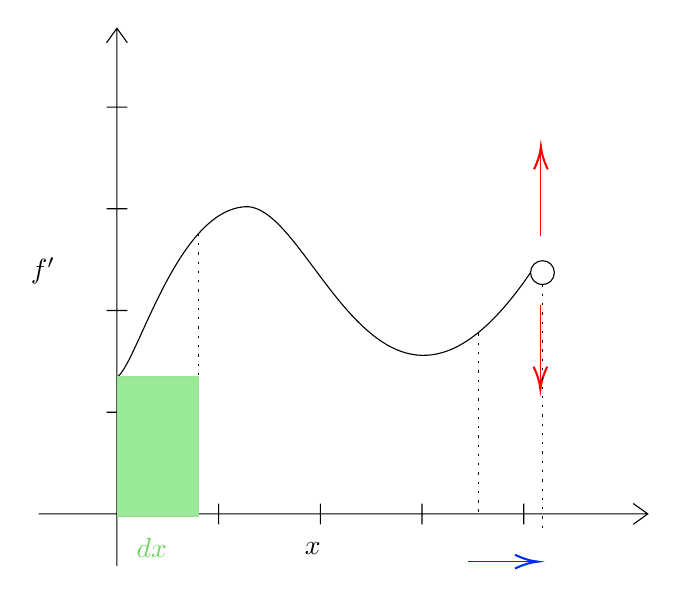
\begin{tikzpicture}[x=0.75pt,y=0.75pt,yscale=-1,xscale=1]
%uncomment if require: \path (0,300); %set diagram left start at 0, and has height of 300

%Shape: Axis 2D [id:dp40268293355011053] 
\draw  (59,251) -- (352.5,251)(96.73,17) -- (96.73,276) (345.5,246) -- (352.5,251) -- (345.5,256) (91.73,24) -- (96.73,17) -- (101.73,24) (145.73,246) -- (145.73,256)(194.73,246) -- (194.73,256)(243.73,246) -- (243.73,256)(292.73,246) -- (292.73,256)(91.73,202) -- (101.73,202)(91.73,153) -- (101.73,153)(91.73,104) -- (101.73,104)(91.73,55) -- (101.73,55) ;
\draw   ;
%Shape: Circle [id:dp27652033411617516] 
\draw   (296,134.75) .. controls (296,131.57) and (298.57,129) .. (301.75,129) .. controls (304.93,129) and (307.5,131.57) .. (307.5,134.75) .. controls (307.5,137.93) and (304.93,140.5) .. (301.75,140.5) .. controls (298.57,140.5) and (296,137.93) .. (296,134.75) -- cycle ;
%Curve Lines [id:da17858959619860293] 
\draw    (97,185) .. controls (106.79,177.66) and (125.5,105) .. (158.5,103) .. controls (191.5,101) and (223.5,241) .. (296,134.75) ;
%Straight Lines [id:da9630299033013741] 
\draw [color={rgb, 255:red, 255; green, 0; blue, 0 }  ,draw opacity=1 ]   (301,117) -- (301,76) ;
\draw [shift={(301,74)}, rotate = 450] [color={rgb, 255:red, 255; green, 0; blue, 0 }  ,draw opacity=1 ][line width=0.75]    (10.93,-3.29) .. controls (6.95,-1.4) and (3.31,-0.3) .. (0,0) .. controls (3.31,0.3) and (6.95,1.4) .. (10.93,3.29)   ;
%Straight Lines [id:da6584610678809868] 
\draw [color={rgb, 255:red, 255; green, 0; blue, 0 }  ,draw opacity=1 ]   (300.75,150.5) -- (300.75,189) ;
\draw [shift={(300.75,191)}, rotate = 270] [color={rgb, 255:red, 255; green, 0; blue, 0 }  ,draw opacity=1 ][line width=0.75]    (10.93,-3.29) .. controls (6.95,-1.4) and (3.31,-0.3) .. (0,0) .. controls (3.31,0.3) and (6.95,1.4) .. (10.93,3.29)   ;
%Straight Lines [id:da3413840183352358] 
\draw  [dash pattern={on 0.84pt off 2.51pt}]  (301.75,140.5) -- (301.75,259) ;
%Straight Lines [id:da3456990383666756] 
\draw [color={rgb, 255:red, 0; green, 42; blue, 255 }  ,draw opacity=1 ]   (266,274) -- (297.5,274) ;
\draw [shift={(299.5,274)}, rotate = 180] [color={rgb, 255:red, 0; green, 42; blue, 255 }  ,draw opacity=1 ][line width=0.75]    (10.93,-3.29) .. controls (6.95,-1.4) and (3.31,-0.3) .. (0,0) .. controls (3.31,0.3) and (6.95,1.4) .. (10.93,3.29)   ;
%Straight Lines [id:da5576696604138862] 
\draw  [dash pattern={on 0.84pt off 2.51pt}]  (271,164) -- (271,250) ;
%Straight Lines [id:da770134158979629] 
\draw  [dash pattern={on 0.84pt off 2.51pt}]  (136,116) -- (136,252) ;
%Shape: Rectangle [id:dp4648872043123744] 
\draw  [color={rgb, 255:red, 151; green, 228; blue, 141 }  ,draw opacity=1 ][fill={rgb, 255:red, 153; green, 233; blue, 153 }  ,fill opacity=1 ] (97,185) -- (136,185) -- (136,252) -- (97,252) -- cycle ;

% Text Node
\draw (54,126.4) node [anchor=north west][inner sep=0.75pt]    {$f'$};
% Text Node
\draw (186,263.4) node [anchor=north west][inner sep=0.75pt]    {$x$};
% Text Node
\draw (105,261.4) node [anchor=north west][inner sep=0.75pt]  [color={rgb, 255:red, 108; green, 211; blue, 99 }  ,opacity=1 ]  {$dx$};


\end{tikzpicture}


If we represent the rate \( f' \) on a graph,
then multiplying the rate by \( dx \) just gives us the area.
Thus the integral is just the area under the rate graph.



\tikzset{every picture/.style={line width=0.75pt}} %set default line width to 0.75pt        
\noindent
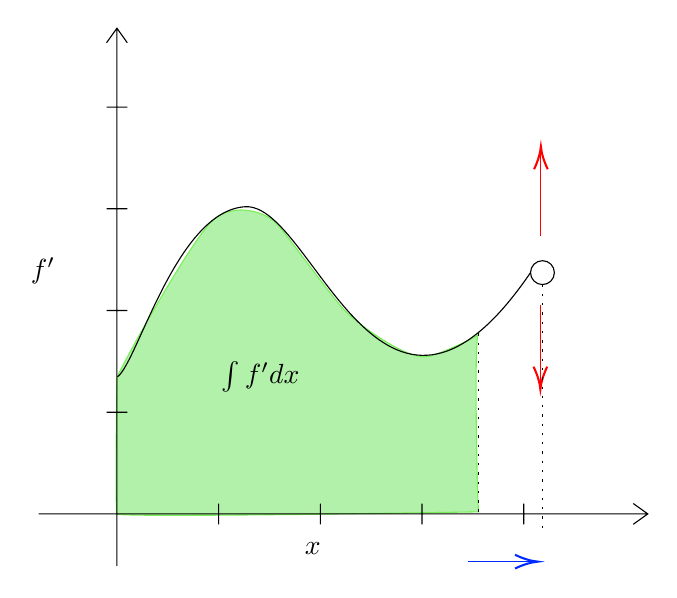
\begin{tikzpicture}[x=0.75pt,y=0.75pt,yscale=-1,xscale=1]
%uncomment if require: \path (0,300); %set diagram left start at 0, and has height of 300

%Shape: Polygon Curved [id:ds4987676772706314] 
\draw  [color={rgb, 255:red, 119; green, 240; blue, 85 }  ,draw opacity=1 ][fill={rgb, 255:red, 177; green, 241; blue, 169 }  ,fill opacity=1 ] (77,186) .. controls (77.5,183) and (113.5,118) .. (123.5,110) .. controls (133.5,102) and (148.5,106) .. (154.5,113) .. controls (160.5,120) and (180.21,147.41) .. (186.5,154) .. controls (192.79,160.59) and (217.5,179) .. (227.5,176) .. controls (237.5,173) and (253.5,165) .. (251,165) .. controls (248.5,165) and (250.5,251) .. (251,251) .. controls (251.5,251) and (77.5,254) .. (76.73,252) .. controls (75.96,250) and (76.5,189) .. (77,186) -- cycle ;
%Shape: Axis 2D [id:dp2444885928490862] 
\draw  (39,252) -- (332.5,252)(76.73,18) -- (76.73,277) (325.5,247) -- (332.5,252) -- (325.5,257) (71.73,25) -- (76.73,18) -- (81.73,25) (125.73,247) -- (125.73,257)(174.73,247) -- (174.73,257)(223.73,247) -- (223.73,257)(272.73,247) -- (272.73,257)(71.73,203) -- (81.73,203)(71.73,154) -- (81.73,154)(71.73,105) -- (81.73,105)(71.73,56) -- (81.73,56) ;
\draw   ;
%Shape: Circle [id:dp4961238584786192] 
\draw   (276,135.75) .. controls (276,132.57) and (278.57,130) .. (281.75,130) .. controls (284.93,130) and (287.5,132.57) .. (287.5,135.75) .. controls (287.5,138.93) and (284.93,141.5) .. (281.75,141.5) .. controls (278.57,141.5) and (276,138.93) .. (276,135.75) -- cycle ;
%Curve Lines [id:da30467668763713107] 
\draw    (77,186) .. controls (86.79,178.66) and (105.5,106) .. (138.5,104) .. controls (171.5,102) and (203.5,242) .. (276,135.75) ;
%Straight Lines [id:da36349385516051635] 
\draw [color={rgb, 255:red, 255; green, 0; blue, 0 }  ,draw opacity=1 ]   (281,118) -- (281,77) ;
\draw [shift={(281,75)}, rotate = 450] [color={rgb, 255:red, 255; green, 0; blue, 0 }  ,draw opacity=1 ][line width=0.75]    (10.93,-3.29) .. controls (6.95,-1.4) and (3.31,-0.3) .. (0,0) .. controls (3.31,0.3) and (6.95,1.4) .. (10.93,3.29)   ;
%Straight Lines [id:da23259457009514273] 
\draw [color={rgb, 255:red, 255; green, 0; blue, 0 }  ,draw opacity=1 ]   (280.75,151.5) -- (280.75,190) ;
\draw [shift={(280.75,192)}, rotate = 270] [color={rgb, 255:red, 255; green, 0; blue, 0 }  ,draw opacity=1 ][line width=0.75]    (10.93,-3.29) .. controls (6.95,-1.4) and (3.31,-0.3) .. (0,0) .. controls (3.31,0.3) and (6.95,1.4) .. (10.93,3.29)   ;
%Straight Lines [id:da3927869746462661] 
\draw  [dash pattern={on 0.84pt off 2.51pt}]  (281.75,141.5) -- (281.75,260) ;
%Straight Lines [id:da5865427634124499] 
\draw [color={rgb, 255:red, 0; green, 42; blue, 255 }  ,draw opacity=1 ]   (246,275) -- (277.5,275) ;
\draw [shift={(279.5,275)}, rotate = 180] [color={rgb, 255:red, 0; green, 42; blue, 255 }  ,draw opacity=1 ][line width=0.75]    (10.93,-3.29) .. controls (6.95,-1.4) and (3.31,-0.3) .. (0,0) .. controls (3.31,0.3) and (6.95,1.4) .. (10.93,3.29)   ;
%Straight Lines [id:da8199987268344746] 
\draw  [dash pattern={on 0.84pt off 2.51pt}]  (251,165) -- (251,251) ;

% Text Node
\draw (34,127.4) node [anchor=north west][inner sep=0.75pt]    {$f'$};
% Text Node
\draw (166,264.4) node [anchor=north west][inner sep=0.75pt]    {$x$};
% Text Node
\draw (126,177.4) node [anchor=north west][inner sep=0.75pt]    {$\int f'dx$};


\end{tikzpicture}



\subsection{\( e \)}

Take some exponential function \( b^t \).
Suppose we want to know how much the function gains per time.
We know that the proportion per time is \( b \).
So the amount of gain is \( b(b^{t}) - b^t = b^t (b - 1) \).
This is just making \( b - 1 \) copies.

\tikzset{every picture/.style={line width=0.75pt}} %set default line width to 0.75pt        
\noindent
\begin{tikzpicture}[x=0.75pt,y=0.75pt,yscale=-1,xscale=1]
%uncomment if require: \path (0,300); %set diagram left start at 0, and has height of 300

%Shape: Axis 2D [id:dp7548955269279164] 
\draw  (34,249) -- (327.5,249)(71.73,15) -- (71.73,274) (320.5,244) -- (327.5,249) -- (320.5,254) (66.73,22) -- (71.73,15) -- (76.73,22) (120.73,244) -- (120.73,254)(169.73,244) -- (169.73,254)(218.73,244) -- (218.73,254)(267.73,244) -- (267.73,254)(66.73,200) -- (76.73,200)(66.73,151) -- (76.73,151)(66.73,102) -- (76.73,102)(66.73,53) -- (76.73,53) ;
\draw   ;
%Shape: Circle [id:dp591863864638757] 
\draw   (270,96.75) .. controls (270,93.57) and (272.57,91) .. (275.75,91) .. controls (278.93,91) and (281.5,93.57) .. (281.5,96.75) .. controls (281.5,99.93) and (278.93,102.5) .. (275.75,102.5) .. controls (272.57,102.5) and (270,99.93) .. (270,96.75) -- cycle ;
%Curve Lines [id:da9965257383628019] 
\draw    (71.73,249) .. controls (91.23,242) and (75.5,211) .. (112.5,194) .. controls (149.5,177) and (180.5,189) .. (207.5,163) .. controls (234.5,137) and (243.5,104) .. (270,96.75) ;
%Straight Lines [id:da4442636779784198] 
\draw [color={rgb, 255:red, 255; green, 0; blue, 0 }  ,draw opacity=1 ]   (275,79) -- (275,38) ;
\draw [shift={(275,36)}, rotate = 450] [color={rgb, 255:red, 255; green, 0; blue, 0 }  ,draw opacity=1 ][line width=0.75]    (10.93,-3.29) .. controls (6.95,-1.4) and (3.31,-0.3) .. (0,0) .. controls (3.31,0.3) and (6.95,1.4) .. (10.93,3.29)   ;
%Straight Lines [id:da7277065515801376] 
\draw [color={rgb, 255:red, 255; green, 0; blue, 0 }  ,draw opacity=1 ]   (274.75,112.5) -- (274.75,151) ;
\draw [shift={(274.75,153)}, rotate = 270] [color={rgb, 255:red, 255; green, 0; blue, 0 }  ,draw opacity=1 ][line width=0.75]    (10.93,-3.29) .. controls (6.95,-1.4) and (3.31,-0.3) .. (0,0) .. controls (3.31,0.3) and (6.95,1.4) .. (10.93,3.29)   ;
%Straight Lines [id:da9297137452591817] 
\draw  [dash pattern={on 0.84pt off 2.51pt}]  (275.75,102.5) -- (275.75,249) ;
%Straight Lines [id:da19635560871451874] 
\draw [color={rgb, 255:red, 0; green, 42; blue, 255 }  ,draw opacity=1 ]   (241,272) -- (272.5,272) ;
\draw [shift={(274.5,272)}, rotate = 180] [color={rgb, 255:red, 0; green, 42; blue, 255 }  ,draw opacity=1 ][line width=0.75]    (10.93,-3.29) .. controls (6.95,-1.4) and (3.31,-0.3) .. (0,0) .. controls (3.31,0.3) and (6.95,1.4) .. (10.93,3.29)   ;
%Shape: Axis 2D [id:dp5159473195200954] 
\draw  (587.2,287.9) -- (587.3,-5.6)(353.21,250.09) -- (612.21,250.18) (582.3,1.4) -- (587.3,-5.6) -- (592.3,1.4) (360.21,255.09) -- (353.21,250.09) -- (360.21,245.09) (582.23,201.17) -- (592.23,201.17)(582.25,152.17) -- (592.25,152.17)(582.26,103.17) -- (592.26,103.17)(582.28,54.17) -- (592.28,54.17)(538.21,255.15) -- (538.21,245.15)(489.21,255.13) -- (489.21,245.13)(440.21,255.12) -- (440.21,245.12)(391.21,255.1) -- (391.21,245.1) ;
\draw   ;
%Shape: Circle [id:dp3595956560062188] 
\draw   (435.03,51.85) .. controls (431.86,51.84) and (429.28,49.27) .. (429.28,46.09) .. controls (429.28,42.92) and (431.86,40.34) .. (435.03,40.35) .. controls (438.21,40.35) and (440.78,42.92) .. (440.78,46.1) .. controls (440.78,49.27) and (438.21,51.85) .. (435.03,51.85) -- cycle ;
%Curve Lines [id:da5301486307360965] 
\draw    (587.21,250.17) .. controls (580.22,230.67) and (549.21,246.39) .. (532.23,209.38) .. controls (515.24,172.37) and (527.25,141.38) .. (501.26,114.37) .. controls (475.27,87.36) and (442.27,78.35) .. (435.03,51.85) ;
%Straight Lines [id:da1701708037395353] 
\draw [color={rgb, 255:red, 255; green, 0; blue, 0 }  ,draw opacity=1 ]   (417.28,46.84) -- (376.28,46.83) ;
\draw [shift={(374.28,46.82)}, rotate = 360.02] [color={rgb, 255:red, 255; green, 0; blue, 0 }  ,draw opacity=1 ][line width=0.75]    (10.93,-3.29) .. controls (6.95,-1.4) and (3.31,-0.3) .. (0,0) .. controls (3.31,0.3) and (6.95,1.4) .. (10.93,3.29)   ;
%Straight Lines [id:da9454232351703403] 
\draw [color={rgb, 255:red, 255; green, 0; blue, 0 }  ,draw opacity=1 ]   (450.78,47.1) -- (489.28,47.12) ;
\draw [shift={(491.28,47.12)}, rotate = 180.02] [color={rgb, 255:red, 255; green, 0; blue, 0 }  ,draw opacity=1 ][line width=0.75]    (10.93,-3.29) .. controls (6.95,-1.4) and (3.31,-0.3) .. (0,0) .. controls (3.31,0.3) and (6.95,1.4) .. (10.93,3.29)   ;
%Straight Lines [id:da6128160114394268] 
\draw  [dash pattern={on 0.84pt off 2.51pt}]  (440.78,46.1) -- (587.28,46.15) ;
%Straight Lines [id:da5100793300598488] 
\draw [color={rgb, 255:red, 0; green, 42; blue, 255 }  ,draw opacity=1 ]   (610.27,80.91) -- (610.28,49.41) ;
\draw [shift={(610.28,47.41)}, rotate = 450.02] [color={rgb, 255:red, 0; green, 42; blue, 255 }  ,draw opacity=1 ][line width=0.75]    (10.93,-3.29) .. controls (6.95,-1.4) and (3.31,-0.3) .. (0,0) .. controls (3.31,0.3) and (6.95,1.4) .. (10.93,3.29)   ;
%Curve Lines [id:da5319468231161516] 
\draw    (367.5,35) .. controls (366.51,-6.58) and (296.91,-9.94) .. (291.64,34.63) ;
\draw [shift={(291.5,36)}, rotate = 274.97] [color={rgb, 255:red, 0; green, 0; blue, 0 }  ][line width=0.75]    (10.93,-3.29) .. controls (6.95,-1.4) and (3.31,-0.3) .. (0,0) .. controls (3.31,0.3) and (6.95,1.4) .. (10.93,3.29)   ;

% Text Node
\draw (28,124.4) node [anchor=north west][inner sep=0.75pt]    {$f$};
% Text Node
\draw (161,261.4) node [anchor=north west][inner sep=0.75pt]    {$x$};
% Text Node
\draw (462.6,293.86) node [anchor=north west][inner sep=0.75pt]  [rotate=-270.02]  {$f$};
% Text Node
\draw (599.64,160.9) node [anchor=north west][inner sep=0.75pt]  [rotate=-270.02]  {$x$};


\end{tikzpicture}

We see that the rate of gain is just a proportion of itself \( (b - 1) \).
So for example, the rate of gain for \( 2^x \) is \( 1 \cdot 2^x = 2^x \).
However, this is a discrete rate (blue).
What if we want the continuous rate? (red).

We define \( e \) such that its continuous rate of growth is 1.
Thus the rate of gain is just \( \dv{x} e^x = 1 \cdot e^x \).


\newpage
\section{Differentiation}


\subsection{Product Rule}

\begin{tikzpicture}[x=0.75pt,y=0.75pt,yscale=-1,xscale=1]
%uncomment if require: \path (0,300); %set diagram left start at 0, and has height of 300

%Shape: Axis 2D [id:dp791486377406529] 
\draw  (50,241.7) -- (314.5,241.7)(76.45,41) -- (76.45,264) (307.5,236.7) -- (314.5,241.7) -- (307.5,246.7) (71.45,48) -- (76.45,41) -- (81.45,48) (115.45,236.7) -- (115.45,246.7)(154.45,236.7) -- (154.45,246.7)(193.45,236.7) -- (193.45,246.7)(232.45,236.7) -- (232.45,246.7)(271.45,236.7) -- (271.45,246.7)(71.45,202.7) -- (81.45,202.7)(71.45,163.7) -- (81.45,163.7)(71.45,124.7) -- (81.45,124.7)(71.45,85.7) -- (81.45,85.7) ;
\draw   ;
%Curve Lines [id:da6119806462814916] 
\draw    (76.45,241.7) .. controls (112.5,67) and (290.5,90) .. (292.5,82) ;
%Shape: Axis 2D [id:dp1956952642703632] 
\draw  (370,238.7) -- (634.5,238.7)(396.45,38) -- (396.45,261) (627.5,233.7) -- (634.5,238.7) -- (627.5,243.7) (391.45,45) -- (396.45,38) -- (401.45,45) (435.45,233.7) -- (435.45,243.7)(474.45,233.7) -- (474.45,243.7)(513.45,233.7) -- (513.45,243.7)(552.45,233.7) -- (552.45,243.7)(591.45,233.7) -- (591.45,243.7)(391.45,199.7) -- (401.45,199.7)(391.45,160.7) -- (401.45,160.7)(391.45,121.7) -- (401.45,121.7)(391.45,82.7) -- (401.45,82.7) ;
\draw   ;
%Curve Lines [id:da6904688712857534] 
\draw    (396.45,238.7) .. controls (432.5,64) and (610.5,87) .. (612.5,79) ;
%Straight Lines [id:da8868203342962732] 
\draw [color={rgb, 255:red, 255; green, 0; blue, 0 }  ,draw opacity=1 ]   (396.45,238.7) -- (429.5,159) ;
%Straight Lines [id:da6732443966151707] 
\draw [color={rgb, 255:red, 255; green, 0; blue, 0 }  ,draw opacity=1 ]   (429.5,159) -- (494.5,105) ;
%Straight Lines [id:da792722354522738] 
\draw [color={rgb, 255:red, 255; green, 0; blue, 0 }  ,draw opacity=1 ]   (600.5,81) -- (494.5,105) ;
%Straight Lines [id:da7780337638207823] 
\draw [color={rgb, 255:red, 0; green, 42; blue, 255 }  ,draw opacity=1 ]   (429.5,159) -- (493.5,159) ;
%Straight Lines [id:da5469718819271276] 
\draw [color={rgb, 255:red, 0; green, 42; blue, 255 }  ,draw opacity=1 ]   (493.5,159) -- (493.5,107) ;

% Text Node
\draw (42,139.4) node [anchor=north west][inner sep=0.75pt]    {$y$};
% Text Node
\draw (174,263.4) node [anchor=north west][inner sep=0.75pt]    {$x$};
% Text Node
\draw (362,136.4) node [anchor=north west][inner sep=0.75pt]    {$y$};
% Text Node
\draw (494,260.4) node [anchor=north west][inner sep=0.75pt]    {$x$};
% Text Node
\draw (454,167.4) node [anchor=north west][inner sep=0.75pt]  [color={rgb, 255:red, 0; green, 95; blue, 255 }  ,opacity=1 ]  {$dx$};
% Text Node
\draw (504,126.4) node [anchor=north west][inner sep=0.75pt]  [color={rgb, 255:red, 0; green, 24; blue, 255 }  ,opacity=1 ]  {$dy$};
% Text Node
\draw (407,75.4) node [anchor=north west][inner sep=0.75pt]  [color={rgb, 255:red, 255; green, 0; blue, 0 }  ,opacity=1 ]  {$\sqrt{dx^{2} +dy^{2}}$};


\end{tikzpicture}

\subsection{Chain}

We run through \( f \) at a rate specified by \( g \).
Thus if we want to convert \( dx \) to \( \dv{f}{x} \)
but we only know \( \dv{f}{g} \),
we just have to multiply by the change in rate of \( g \)


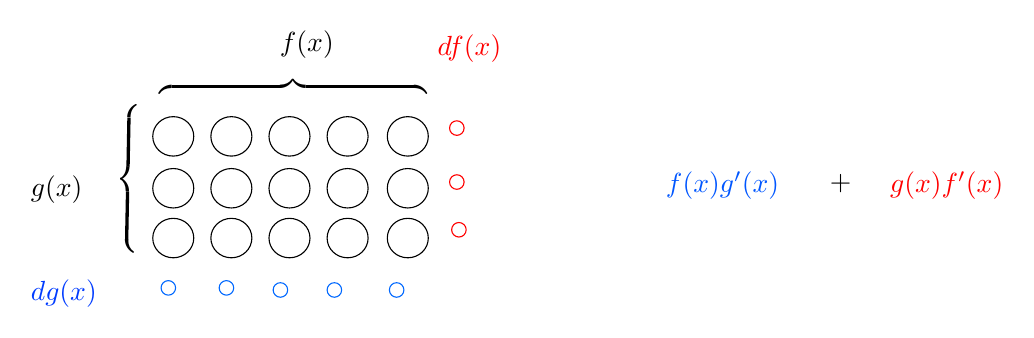
\begin{tikzpicture}[x=0.75pt,y=0.75pt,yscale=-1,xscale=1]
%uncomment if require: \path (0,300); %set diagram left start at 0, and has height of 300

%Shape: Ellipse [id:dp06031973450750061] 
\draw   (164,126.5) .. controls (164,121.25) and (168.42,117) .. (173.88,117) .. controls (179.33,117) and (183.75,121.25) .. (183.75,126.5) .. controls (183.75,131.75) and (179.33,136) .. (173.88,136) .. controls (168.42,136) and (164,131.75) .. (164,126.5) -- cycle ;
%Shape: Ellipse [id:dp8478408655553544] 
\draw   (192,126.5) .. controls (192,121.25) and (196.42,117) .. (201.88,117) .. controls (207.33,117) and (211.75,121.25) .. (211.75,126.5) .. controls (211.75,131.75) and (207.33,136) .. (201.88,136) .. controls (196.42,136) and (192,131.75) .. (192,126.5) -- cycle ;
%Shape: Ellipse [id:dp505421117341947] 
\draw   (220,126.5) .. controls (220,121.25) and (224.42,117) .. (229.88,117) .. controls (235.33,117) and (239.75,121.25) .. (239.75,126.5) .. controls (239.75,131.75) and (235.33,136) .. (229.88,136) .. controls (224.42,136) and (220,131.75) .. (220,126.5) -- cycle ;
%Shape: Ellipse [id:dp007218742660141997] 
\draw   (248,126.5) .. controls (248,121.25) and (252.42,117) .. (257.88,117) .. controls (263.33,117) and (267.75,121.25) .. (267.75,126.5) .. controls (267.75,131.75) and (263.33,136) .. (257.88,136) .. controls (252.42,136) and (248,131.75) .. (248,126.5) -- cycle ;
%Shape: Ellipse [id:dp8702465733669611] 
\draw   (277,126.5) .. controls (277,121.25) and (281.42,117) .. (286.88,117) .. controls (292.33,117) and (296.75,121.25) .. (296.75,126.5) .. controls (296.75,131.75) and (292.33,136) .. (286.88,136) .. controls (281.42,136) and (277,131.75) .. (277,126.5) -- cycle ;
%Shape: Ellipse [id:dp6716570870833466] 
\draw   (164,151.5) .. controls (164,146.25) and (168.42,142) .. (173.88,142) .. controls (179.33,142) and (183.75,146.25) .. (183.75,151.5) .. controls (183.75,156.75) and (179.33,161) .. (173.88,161) .. controls (168.42,161) and (164,156.75) .. (164,151.5) -- cycle ;
%Shape: Ellipse [id:dp1820921953890161] 
\draw   (192,151.5) .. controls (192,146.25) and (196.42,142) .. (201.88,142) .. controls (207.33,142) and (211.75,146.25) .. (211.75,151.5) .. controls (211.75,156.75) and (207.33,161) .. (201.88,161) .. controls (196.42,161) and (192,156.75) .. (192,151.5) -- cycle ;
%Shape: Ellipse [id:dp5866793827026061] 
\draw   (220,151.5) .. controls (220,146.25) and (224.42,142) .. (229.88,142) .. controls (235.33,142) and (239.75,146.25) .. (239.75,151.5) .. controls (239.75,156.75) and (235.33,161) .. (229.88,161) .. controls (224.42,161) and (220,156.75) .. (220,151.5) -- cycle ;
%Shape: Ellipse [id:dp45797332679454195] 
\draw   (248,151.5) .. controls (248,146.25) and (252.42,142) .. (257.88,142) .. controls (263.33,142) and (267.75,146.25) .. (267.75,151.5) .. controls (267.75,156.75) and (263.33,161) .. (257.88,161) .. controls (252.42,161) and (248,156.75) .. (248,151.5) -- cycle ;
%Shape: Ellipse [id:dp24430516488734677] 
\draw   (277,151.5) .. controls (277,146.25) and (281.42,142) .. (286.88,142) .. controls (292.33,142) and (296.75,146.25) .. (296.75,151.5) .. controls (296.75,156.75) and (292.33,161) .. (286.88,161) .. controls (281.42,161) and (277,156.75) .. (277,151.5) -- cycle ;
%Shape: Ellipse [id:dp5662108764983852] 
\draw   (164,175.5) .. controls (164,170.25) and (168.42,166) .. (173.88,166) .. controls (179.33,166) and (183.75,170.25) .. (183.75,175.5) .. controls (183.75,180.75) and (179.33,185) .. (173.88,185) .. controls (168.42,185) and (164,180.75) .. (164,175.5) -- cycle ;
%Shape: Ellipse [id:dp6579543801408282] 
\draw   (192,175.5) .. controls (192,170.25) and (196.42,166) .. (201.88,166) .. controls (207.33,166) and (211.75,170.25) .. (211.75,175.5) .. controls (211.75,180.75) and (207.33,185) .. (201.88,185) .. controls (196.42,185) and (192,180.75) .. (192,175.5) -- cycle ;
%Shape: Ellipse [id:dp17883475704623442] 
\draw   (220,175.5) .. controls (220,170.25) and (224.42,166) .. (229.88,166) .. controls (235.33,166) and (239.75,170.25) .. (239.75,175.5) .. controls (239.75,180.75) and (235.33,185) .. (229.88,185) .. controls (224.42,185) and (220,180.75) .. (220,175.5) -- cycle ;
%Shape: Ellipse [id:dp8959152379599131] 
\draw   (248,175.5) .. controls (248,170.25) and (252.42,166) .. (257.88,166) .. controls (263.33,166) and (267.75,170.25) .. (267.75,175.5) .. controls (267.75,180.75) and (263.33,185) .. (257.88,185) .. controls (252.42,185) and (248,180.75) .. (248,175.5) -- cycle ;
%Shape: Ellipse [id:dp8976107913184502] 
\draw   (277,175.5) .. controls (277,170.25) and (281.42,166) .. (286.88,166) .. controls (292.33,166) and (296.75,170.25) .. (296.75,175.5) .. controls (296.75,180.75) and (292.33,185) .. (286.88,185) .. controls (281.42,185) and (277,180.75) .. (277,175.5) -- cycle ;
%Shape: Circle [id:dp01856382719091243] 
\draw  [color={rgb, 255:red, 255; green, 0; blue, 0 }  ,draw opacity=1 ] (307,122.5) .. controls (307,120.57) and (308.57,119) .. (310.5,119) .. controls (312.43,119) and (314,120.57) .. (314,122.5) .. controls (314,124.43) and (312.43,126) .. (310.5,126) .. controls (308.57,126) and (307,124.43) .. (307,122.5) -- cycle ;
%Shape: Circle [id:dp4403664682847295] 
\draw  [color={rgb, 255:red, 0; green, 104; blue, 255 }  ,draw opacity=1 ] (168,199.5) .. controls (168,197.57) and (169.57,196) .. (171.5,196) .. controls (173.43,196) and (175,197.57) .. (175,199.5) .. controls (175,201.43) and (173.43,203) .. (171.5,203) .. controls (169.57,203) and (168,201.43) .. (168,199.5) -- cycle ;
%Shape: Circle [id:dp07179694909069678] 
\draw  [color={rgb, 255:red, 0; green, 104; blue, 255 }  ,draw opacity=1 ] (196,199.5) .. controls (196,197.57) and (197.57,196) .. (199.5,196) .. controls (201.43,196) and (203,197.57) .. (203,199.5) .. controls (203,201.43) and (201.43,203) .. (199.5,203) .. controls (197.57,203) and (196,201.43) .. (196,199.5) -- cycle ;
%Shape: Circle [id:dp1451673451815234] 
\draw  [color={rgb, 255:red, 0; green, 104; blue, 255 }  ,draw opacity=1 ] (222,200.5) .. controls (222,198.57) and (223.57,197) .. (225.5,197) .. controls (227.43,197) and (229,198.57) .. (229,200.5) .. controls (229,202.43) and (227.43,204) .. (225.5,204) .. controls (223.57,204) and (222,202.43) .. (222,200.5) -- cycle ;
%Shape: Circle [id:dp9161876920152885] 
\draw  [color={rgb, 255:red, 0; green, 104; blue, 255 }  ,draw opacity=1 ] (248,200.5) .. controls (248,198.57) and (249.57,197) .. (251.5,197) .. controls (253.43,197) and (255,198.57) .. (255,200.5) .. controls (255,202.43) and (253.43,204) .. (251.5,204) .. controls (249.57,204) and (248,202.43) .. (248,200.5) -- cycle ;
%Shape: Circle [id:dp7144565199430419] 
\draw  [color={rgb, 255:red, 0; green, 104; blue, 255 }  ,draw opacity=1 ] (278,200.5) .. controls (278,198.57) and (279.57,197) .. (281.5,197) .. controls (283.43,197) and (285,198.57) .. (285,200.5) .. controls (285,202.43) and (283.43,204) .. (281.5,204) .. controls (279.57,204) and (278,202.43) .. (278,200.5) -- cycle ;
%Shape: Circle [id:dp8377649456481785] 
\draw  [color={rgb, 255:red, 255; green, 0; blue, 0 }  ,draw opacity=1 ] (307,148.5) .. controls (307,146.57) and (308.57,145) .. (310.5,145) .. controls (312.43,145) and (314,146.57) .. (314,148.5) .. controls (314,150.43) and (312.43,152) .. (310.5,152) .. controls (308.57,152) and (307,150.43) .. (307,148.5) -- cycle ;
%Shape: Circle [id:dp940388133671272] 
\draw  [color={rgb, 255:red, 255; green, 0; blue, 0 }  ,draw opacity=1 ] (308,171.5) .. controls (308,169.57) and (309.57,168) .. (311.5,168) .. controls (313.43,168) and (315,169.57) .. (315,171.5) .. controls (315,173.43) and (313.43,175) .. (311.5,175) .. controls (309.57,175) and (308,173.43) .. (308,171.5) -- cycle ;

% Text Node
\draw (224,74.4) node [anchor=north west][inner sep=0.75pt]    {$f( x)$};
% Text Node
\draw (166,96.4) node [anchor=north west][inner sep=0.75pt]    {$\overbrace{\ \ \ \ \ \ \ \ \ \ \ \ \ \ \ \ \ \ \ \ \ \ \ \ \ \ \ \ \ }$};
% Text Node
\draw (145.21,183.74) node [anchor=north west][inner sep=0.75pt]  [rotate=-271.09]  {$\overbrace{\ \ \ \ \ \ \ \ \ \ \ \ \ \ \ \ }$};
% Text Node
\draw (104,144.4) node [anchor=north west][inner sep=0.75pt]    {$g( x)$};
% Text Node
\draw (300,76.4) node [anchor=north west][inner sep=0.75pt]  [color={rgb, 255:red, 255; green, 0; blue, 0 }  ,opacity=1 ]  {$df( x)$};
% Text Node
\draw (104,194.4) node [anchor=north west][inner sep=0.75pt]  [color={rgb, 255:red, 0; green, 59; blue, 255 }  ,opacity=1 ]  {$dg( x)$};
% Text Node
\draw (410,142.4) node [anchor=north west][inner sep=0.75pt]  [color={rgb, 255:red, 0; green, 86; blue, 255 }  ,opacity=1 ]  {$f( x) g'( x)$};
% Text Node
\draw (489,143.4) node [anchor=north west][inner sep=0.75pt]    {$+$};
% Text Node
\draw (518,142.4) node [anchor=north west][inner sep=0.75pt]  [color={rgb, 255:red, 255; green, 0; blue, 0 }  ,opacity=1 ]  {$g( x) f'( x)$};


\end{tikzpicture}

\( \dv{x} f(g) = f'(g)g' \)

\subsection{Reciprocol}

\( \dv{x} \frac{1}{x} = - \frac{1}{x} \cdot \frac{1}{x} = - \frac{1}{x^2} \)


\tikzset{every picture/.style={line width=0.75pt}} %set default line width to 0.75pt        
\noindent
\begin{tikzpicture}[x=0.75pt,y=0.75pt,yscale=-1,xscale=1]
%uncomment if require: \path (0,300); %set diagram left start at 0, and has height of 300

%Shape: Axis 2D [id:dp7548955269279164] 
\draw  (34,249) -- (327.5,249)(71.73,15) -- (71.73,274) (320.5,244) -- (327.5,249) -- (320.5,254) (66.73,22) -- (71.73,15) -- (76.73,22) (120.73,244) -- (120.73,254)(169.73,244) -- (169.73,254)(218.73,244) -- (218.73,254)(267.73,244) -- (267.73,254)(66.73,200) -- (76.73,200)(66.73,151) -- (76.73,151)(66.73,102) -- (76.73,102)(66.73,53) -- (76.73,53) ;
\draw   ;
%Shape: Circle [id:dp591863864638757] 
\draw   (270,96.75) .. controls (270,93.57) and (272.57,91) .. (275.75,91) .. controls (278.93,91) and (281.5,93.57) .. (281.5,96.75) .. controls (281.5,99.93) and (278.93,102.5) .. (275.75,102.5) .. controls (272.57,102.5) and (270,99.93) .. (270,96.75) -- cycle ;
%Curve Lines [id:da9965257383628019] 
\draw    (71.73,249) .. controls (91.23,242) and (75.5,211) .. (112.5,194) .. controls (149.5,177) and (180.5,189) .. (207.5,163) .. controls (234.5,137) and (243.5,104) .. (270,96.75) ;
%Straight Lines [id:da4442636779784198] 
\draw [color={rgb, 255:red, 255; green, 0; blue, 0 }  ,draw opacity=1 ]   (275,79) -- (275,38) ;
\draw [shift={(275,36)}, rotate = 450] [color={rgb, 255:red, 255; green, 0; blue, 0 }  ,draw opacity=1 ][line width=0.75]    (10.93,-3.29) .. controls (6.95,-1.4) and (3.31,-0.3) .. (0,0) .. controls (3.31,0.3) and (6.95,1.4) .. (10.93,3.29)   ;
%Straight Lines [id:da7277065515801376] 
\draw [color={rgb, 255:red, 255; green, 0; blue, 0 }  ,draw opacity=1 ]   (274.75,112.5) -- (274.75,151) ;
\draw [shift={(274.75,153)}, rotate = 270] [color={rgb, 255:red, 255; green, 0; blue, 0 }  ,draw opacity=1 ][line width=0.75]    (10.93,-3.29) .. controls (6.95,-1.4) and (3.31,-0.3) .. (0,0) .. controls (3.31,0.3) and (6.95,1.4) .. (10.93,3.29)   ;
%Straight Lines [id:da9297137452591817] 
\draw  [dash pattern={on 0.84pt off 2.51pt}]  (275.75,102.5) -- (275.75,249) ;
%Straight Lines [id:da19635560871451874] 
\draw [color={rgb, 255:red, 0; green, 42; blue, 255 }  ,draw opacity=1 ]   (241,272) -- (272.5,272) ;
\draw [shift={(274.5,272)}, rotate = 180] [color={rgb, 255:red, 0; green, 42; blue, 255 }  ,draw opacity=1 ][line width=0.75]    (10.93,-3.29) .. controls (6.95,-1.4) and (3.31,-0.3) .. (0,0) .. controls (3.31,0.3) and (6.95,1.4) .. (10.93,3.29)   ;
%Shape: Axis 2D [id:dp5159473195200954] 
\draw  (587.2,287.9) -- (587.3,-5.6)(353.21,250.09) -- (612.21,250.18) (582.3,1.4) -- (587.3,-5.6) -- (592.3,1.4) (360.21,255.09) -- (353.21,250.09) -- (360.21,245.09) (582.23,201.17) -- (592.23,201.17)(582.25,152.17) -- (592.25,152.17)(582.26,103.17) -- (592.26,103.17)(582.28,54.17) -- (592.28,54.17)(538.21,255.15) -- (538.21,245.15)(489.21,255.13) -- (489.21,245.13)(440.21,255.12) -- (440.21,245.12)(391.21,255.1) -- (391.21,245.1) ;
\draw   ;
%Shape: Circle [id:dp3595956560062188] 
\draw   (435.03,51.85) .. controls (431.86,51.84) and (429.28,49.27) .. (429.28,46.09) .. controls (429.28,42.92) and (431.86,40.34) .. (435.03,40.35) .. controls (438.21,40.35) and (440.78,42.92) .. (440.78,46.1) .. controls (440.78,49.27) and (438.21,51.85) .. (435.03,51.85) -- cycle ;
%Curve Lines [id:da5301486307360965] 
\draw    (587.21,250.17) .. controls (580.22,230.67) and (549.21,246.39) .. (532.23,209.38) .. controls (515.24,172.37) and (527.25,141.38) .. (501.26,114.37) .. controls (475.27,87.36) and (442.27,78.35) .. (435.03,51.85) ;
%Straight Lines [id:da1701708037395353] 
\draw [color={rgb, 255:red, 255; green, 0; blue, 0 }  ,draw opacity=1 ]   (417.28,46.84) -- (376.28,46.83) ;
\draw [shift={(374.28,46.82)}, rotate = 360.02] [color={rgb, 255:red, 255; green, 0; blue, 0 }  ,draw opacity=1 ][line width=0.75]    (10.93,-3.29) .. controls (6.95,-1.4) and (3.31,-0.3) .. (0,0) .. controls (3.31,0.3) and (6.95,1.4) .. (10.93,3.29)   ;
%Straight Lines [id:da9454232351703403] 
\draw [color={rgb, 255:red, 255; green, 0; blue, 0 }  ,draw opacity=1 ]   (450.78,47.1) -- (489.28,47.12) ;
\draw [shift={(491.28,47.12)}, rotate = 180.02] [color={rgb, 255:red, 255; green, 0; blue, 0 }  ,draw opacity=1 ][line width=0.75]    (10.93,-3.29) .. controls (6.95,-1.4) and (3.31,-0.3) .. (0,0) .. controls (3.31,0.3) and (6.95,1.4) .. (10.93,3.29)   ;
%Straight Lines [id:da6128160114394268] 
\draw  [dash pattern={on 0.84pt off 2.51pt}]  (440.78,46.1) -- (587.28,46.15) ;
%Straight Lines [id:da5100793300598488] 
\draw [color={rgb, 255:red, 0; green, 42; blue, 255 }  ,draw opacity=1 ]   (610.27,80.91) -- (610.28,49.41) ;
\draw [shift={(610.28,47.41)}, rotate = 450.02] [color={rgb, 255:red, 0; green, 42; blue, 255 }  ,draw opacity=1 ][line width=0.75]    (10.93,-3.29) .. controls (6.95,-1.4) and (3.31,-0.3) .. (0,0) .. controls (3.31,0.3) and (6.95,1.4) .. (10.93,3.29)   ;
%Curve Lines [id:da5319468231161516] 
\draw    (367.5,35) .. controls (366.51,-6.58) and (296.91,-9.94) .. (291.64,34.63) ;
\draw [shift={(291.5,36)}, rotate = 274.97] [color={rgb, 255:red, 0; green, 0; blue, 0 }  ][line width=0.75]    (10.93,-3.29) .. controls (6.95,-1.4) and (3.31,-0.3) .. (0,0) .. controls (3.31,0.3) and (6.95,1.4) .. (10.93,3.29)   ;

% Text Node
\draw (28,124.4) node [anchor=north west][inner sep=0.75pt]    {$f$};
% Text Node
\draw (161,261.4) node [anchor=north west][inner sep=0.75pt]    {$x$};
% Text Node
\draw (462.6,293.86) node [anchor=north west][inner sep=0.75pt]  [rotate=-270.02]  {$f$};
% Text Node
\draw (599.64,160.9) node [anchor=north west][inner sep=0.75pt]  [rotate=-270.02]  {$x$};


\end{tikzpicture}

\subsection{Quotient}

\( \dv{x} fg^{-1} = f'g^{-1} - fg^{-2}g' = \frac{f'g - fg'}{g^2} \)

\subsection{exp and log}

We know \( \dv{x} b^x = ab^x \) where \( a \) is some proportion.
We also know that \( b^x = e^{\ln(b) x} \) so
\[ \dv{x} b^x = b^x \dv{x} \ln(b) x = b^x \ln(b) \]
Thus \( a = \ln(b) \).

At some proportion \( e^x \), our rate of growth is \( e^x \).
If we take the inverse \( \ln(x) \), then instead of multiplying, we divide.
so \( \dv{x} \ln(x) = \frac{1}{x} \).

\subsection{Inverse}

Recall that composition is taking a functions domain \( x \),
and instead of moving through it at a rate of 1 per \( x \),
we go through it at a rate dictated by some other function \( g(x) \).

\noindent
\begin{tikzpicture}[x=0.75pt,y=0.75pt,yscale=-1,xscale=1]
%uncomment if require: \path (0,300); %set diagram left start at 0, and has height of 300

%Shape: Axis 2D [id:dp3419332376667883] 
\draw  (41,249) -- (334.5,249)(78.73,15) -- (78.73,274) (327.5,244) -- (334.5,249) -- (327.5,254) (73.73,22) -- (78.73,15) -- (83.73,22) (127.73,244) -- (127.73,254)(176.73,244) -- (176.73,254)(225.73,244) -- (225.73,254)(274.73,244) -- (274.73,254)(73.73,200) -- (83.73,200)(73.73,151) -- (83.73,151)(73.73,102) -- (83.73,102)(73.73,53) -- (83.73,53) ;
\draw   ;
%Shape: Circle [id:dp15714841919076528] 
\draw   (278,132.75) .. controls (278,129.57) and (280.57,127) .. (283.75,127) .. controls (286.93,127) and (289.5,129.57) .. (289.5,132.75) .. controls (289.5,135.93) and (286.93,138.5) .. (283.75,138.5) .. controls (280.57,138.5) and (278,135.93) .. (278,132.75) -- cycle ;
%Curve Lines [id:da48902714333738084] 
\draw    (79,183) .. controls (88.79,175.66) and (92.03,119.89) .. (120.27,166.95) .. controls (148.5,214) and (187.02,172.39) .. (223.5,199) .. controls (259.98,225.61) and (248.5,129) .. (278,132.75) ;
%Straight Lines [id:da8141145633432557] 
\draw [color={rgb, 255:red, 255; green, 0; blue, 0 }  ,draw opacity=1 ]   (283,115) -- (283,74) ;
\draw [shift={(283,72)}, rotate = 450] [color={rgb, 255:red, 255; green, 0; blue, 0 }  ,draw opacity=1 ][line width=0.75]    (10.93,-3.29) .. controls (6.95,-1.4) and (3.31,-0.3) .. (0,0) .. controls (3.31,0.3) and (6.95,1.4) .. (10.93,3.29)   ;
%Straight Lines [id:da3154003786291655] 
\draw [color={rgb, 255:red, 255; green, 0; blue, 0 }  ,draw opacity=1 ]   (282.75,148.5) -- (282.75,187) ;
\draw [shift={(282.75,189)}, rotate = 270] [color={rgb, 255:red, 255; green, 0; blue, 0 }  ,draw opacity=1 ][line width=0.75]    (10.93,-3.29) .. controls (6.95,-1.4) and (3.31,-0.3) .. (0,0) .. controls (3.31,0.3) and (6.95,1.4) .. (10.93,3.29)   ;
%Straight Lines [id:da19276906577043762] 
\draw  [dash pattern={on 0.84pt off 2.51pt}]  (283.75,138.5) -- (283.75,257) ;
%Straight Lines [id:da9895246969397727] 
\draw [color={rgb, 255:red, 0; green, 42; blue, 255 }  ,draw opacity=1 ]   (248,272) -- (279.5,272) ;
\draw [shift={(281.5,272)}, rotate = 180] [color={rgb, 255:red, 0; green, 42; blue, 255 }  ,draw opacity=1 ][line width=0.75]    (10.93,-3.29) .. controls (6.95,-1.4) and (3.31,-0.3) .. (0,0) .. controls (3.31,0.3) and (6.95,1.4) .. (10.93,3.29)   ;
%Shape: Axis 2D [id:dp074444405148542] 
\draw  (338,248) -- (631.5,248)(375.73,14) -- (375.73,273) (624.5,243) -- (631.5,248) -- (624.5,253) (370.73,21) -- (375.73,14) -- (380.73,21) (424.73,243) -- (424.73,253)(473.73,243) -- (473.73,253)(522.73,243) -- (522.73,253)(571.73,243) -- (571.73,253)(370.73,199) -- (380.73,199)(370.73,150) -- (380.73,150)(370.73,101) -- (380.73,101)(370.73,52) -- (380.73,52) ;
\draw   ;
%Shape: Circle [id:dp6593224815387302] 
\draw   (575,131.75) .. controls (575,128.57) and (577.57,126) .. (580.75,126) .. controls (583.93,126) and (586.5,128.57) .. (586.5,131.75) .. controls (586.5,134.93) and (583.93,137.5) .. (580.75,137.5) .. controls (577.57,137.5) and (575,134.93) .. (575,131.75) -- cycle ;
%Curve Lines [id:da4000391883296601] 
\draw    (376,182) .. controls (385.79,174.66) and (412.27,121.95) .. (440.5,169) .. controls (468.73,216.05) and (458.02,173.39) .. (494.5,200) .. controls (530.98,226.61) and (540.5,199) .. (575,131.75) ;
%Straight Lines [id:da6430080624749632] 
\draw [color={rgb, 255:red, 255; green, 0; blue, 0 }  ,draw opacity=1 ]   (580,114) -- (580,73) ;
\draw [shift={(580,71)}, rotate = 450] [color={rgb, 255:red, 255; green, 0; blue, 0 }  ,draw opacity=1 ][line width=0.75]    (10.93,-3.29) .. controls (6.95,-1.4) and (3.31,-0.3) .. (0,0) .. controls (3.31,0.3) and (6.95,1.4) .. (10.93,3.29)   ;
%Straight Lines [id:da3118969368266129] 
\draw [color={rgb, 255:red, 255; green, 0; blue, 0 }  ,draw opacity=1 ]   (579.75,147.5) -- (579.75,186) ;
\draw [shift={(579.75,188)}, rotate = 270] [color={rgb, 255:red, 255; green, 0; blue, 0 }  ,draw opacity=1 ][line width=0.75]    (10.93,-3.29) .. controls (6.95,-1.4) and (3.31,-0.3) .. (0,0) .. controls (3.31,0.3) and (6.95,1.4) .. (10.93,3.29)   ;
%Straight Lines [id:da9742164918890941] 
\draw  [dash pattern={on 0.84pt off 2.51pt}]  (580.75,137.5) -- (580.75,256) ;
%Straight Lines [id:da590167212523919] 
\draw [color={rgb, 255:red, 0; green, 42; blue, 255 }  ,draw opacity=1 ]   (545,271) -- (576.5,271) ;
\draw [shift={(578.5,271)}, rotate = 180] [color={rgb, 255:red, 0; green, 42; blue, 255 }  ,draw opacity=1 ][line width=0.75]    (10.93,-3.29) .. controls (6.95,-1.4) and (3.31,-0.3) .. (0,0) .. controls (3.31,0.3) and (6.95,1.4) .. (10.93,3.29)   ;

% Text Node
\draw (35,124.4) node [anchor=north west][inner sep=0.75pt]    {$f$};
% Text Node
\draw (168,261.4) node [anchor=north west][inner sep=0.75pt]    {$x$};
% Text Node
\draw (332,123.4) node [anchor=north west][inner sep=0.75pt]    {$f$};
% Text Node
\draw (468,263.4) node [anchor=north west][inner sep=0.75pt]    {$x$};
% Text Node
\draw (547,274.4) node [anchor=north west][inner sep=0.75pt]    {$g( x)$};


\end{tikzpicture}


The rate \( \dv{g}{x} \) is just \( g'(x) \).
To convert from \( x \) to \( g \), we just multiply by the rate.
Take \( g\inv: g(x) \to x \) to be the inverse which reverses the process.

\noindent
\tikzset{every picture/.style={line width=0.75pt}} %set default line width to 0.75pt        
\noindent
\begin{tikzpicture}[x=0.75pt,y=0.75pt,yscale=-1,xscale=1]
%uncomment if require: \path (0,300); %set diagram left start at 0, and has height of 300

%Straight Lines [id:da7431716710742607] 
\draw [color={rgb, 255:red, 0; green, 59; blue, 255 }  ,draw opacity=1 ]   (326.5,175.75) -- (397.5,175.75) ;
\draw [shift={(399.5,175.75)}, rotate = 180] [color={rgb, 255:red, 0; green, 59; blue, 255 }  ,draw opacity=1 ][line width=0.75]    (10.93,-3.29) .. controls (6.95,-1.4) and (3.31,-0.3) .. (0,0) .. controls (3.31,0.3) and (6.95,1.4) .. (10.93,3.29)   ;
%Shape: Circle [id:dp9644160811796276] 
\draw  [color={rgb, 255:red, 0; green, 33; blue, 255 }  ,draw opacity=1 ] (317.75,142.75) .. controls (317.75,119.14) and (336.89,100) .. (360.5,100) .. controls (384.11,100) and (403.25,119.14) .. (403.25,142.75) .. controls (403.25,166.36) and (384.11,185.5) .. (360.5,185.5) .. controls (336.89,185.5) and (317.75,166.36) .. (317.75,142.75) -- cycle ;
%Curve Lines [id:da3240856205395106] 
\draw    (284.5,190.5) .. controls (332.5,186.5) and (366.5,115.5) .. (432.5,114.5) ;
%Straight Lines [id:da874388198033234] 
\draw [color={rgb, 255:red, 255; green, 0; blue, 0 }  ,draw opacity=1 ]   (397.5,175.75) -- (397.5,130.75) ;
\draw [shift={(397.5,128.75)}, rotate = 450] [color={rgb, 255:red, 255; green, 0; blue, 0 }  ,draw opacity=1 ][line width=0.75]    (10.93,-3.29) .. controls (6.95,-1.4) and (3.31,-0.3) .. (0,0) .. controls (3.31,0.3) and (6.95,1.4) .. (10.93,3.29)   ;
%Straight Lines [id:da45029407338403327] 
\draw [color={rgb, 255:red, 0; green, 59; blue, 255 }  ,draw opacity=1 ]   (531.5,162.75) -- (560.5,162.75) ;
\draw [shift={(562.5,162.75)}, rotate = 180] [color={rgb, 255:red, 0; green, 59; blue, 255 }  ,draw opacity=1 ][line width=0.75]    (10.93,-3.29) .. controls (6.95,-1.4) and (3.31,-0.3) .. (0,0) .. controls (3.31,0.3) and (6.95,1.4) .. (10.93,3.29)   ;
%Shape: Circle [id:dp6907913190401643] 
\draw  [color={rgb, 255:red, 0; green, 33; blue, 255 }  ,draw opacity=1 ] (528.63,145.13) .. controls (528.63,134.42) and (537.3,125.75) .. (548,125.75) .. controls (558.7,125.75) and (567.38,134.42) .. (567.38,145.13) .. controls (567.38,155.83) and (558.7,164.5) .. (548,164.5) .. controls (537.3,164.5) and (528.63,155.83) .. (528.63,145.13) -- cycle ;
%Curve Lines [id:da7813152440439562] 
\draw    (471.5,189.5) .. controls (519.5,185.5) and (553.5,114.5) .. (619.5,113.5) ;
%Straight Lines [id:da4446042787516894] 
\draw [color={rgb, 255:red, 255; green, 0; blue, 0 }  ,draw opacity=1 ]   (562.5,162.75) -- (562.5,140.75) ;
\draw [shift={(562.5,138.75)}, rotate = 450] [color={rgb, 255:red, 255; green, 0; blue, 0 }  ,draw opacity=1 ][line width=0.75]    (10.93,-3.29) .. controls (6.95,-1.4) and (3.31,-0.3) .. (0,0) .. controls (3.31,0.3) and (6.95,1.4) .. (10.93,3.29)   ;
%Straight Lines [id:da8689576118431565] 
\draw [color={rgb, 255:red, 0; green, 59; blue, 255 }  ,draw opacity=1 ]   (41.5,202.75) -- (190.5,202.75) ;
\draw [shift={(192.5,202.75)}, rotate = 180] [color={rgb, 255:red, 0; green, 59; blue, 255 }  ,draw opacity=1 ][line width=0.75]    (10.93,-3.29) .. controls (6.95,-1.4) and (3.31,-0.3) .. (0,0) .. controls (3.31,0.3) and (6.95,1.4) .. (10.93,3.29)   ;
%Shape: Circle [id:dp15051410322467185] 
\draw  [color={rgb, 255:red, 0; green, 33; blue, 255 }  ,draw opacity=1 ] (29,156.25) .. controls (29,109.72) and (66.72,72) .. (113.25,72) .. controls (159.78,72) and (197.5,109.72) .. (197.5,156.25) .. controls (197.5,202.78) and (159.78,240.5) .. (113.25,240.5) .. controls (66.72,240.5) and (29,202.78) .. (29,156.25) -- cycle ;
%Curve Lines [id:da20936258103749295] 
\draw    (41.5,197) .. controls (89.5,193) and (123.5,122) .. (189.5,121) ;
%Straight Lines [id:da8584771026489159] 
\draw [color={rgb, 255:red, 255; green, 0; blue, 0 }  ,draw opacity=1 ]   (189.5,202.75) -- (189.5,128.75) ;
\draw [shift={(189.5,126.75)}, rotate = 450] [color={rgb, 255:red, 255; green, 0; blue, 0 }  ,draw opacity=1 ][line width=0.75]    (10.93,-3.29) .. controls (6.95,-1.4) and (3.31,-0.3) .. (0,0) .. controls (3.31,0.3) and (6.95,1.4) .. (10.93,3.29)   ;
%Shape: Circle [id:dp7775919650361445] 
\draw   (35.75,197) .. controls (35.75,193.82) and (38.32,191.25) .. (41.5,191.25) .. controls (44.68,191.25) and (47.25,193.82) .. (47.25,197) .. controls (47.25,200.18) and (44.68,202.75) .. (41.5,202.75) .. controls (38.32,202.75) and (35.75,200.18) .. (35.75,197) -- cycle ;
%Shape: Circle [id:dp8539055538820641] 
\draw   (183.75,121) .. controls (183.75,117.82) and (186.32,115.25) .. (189.5,115.25) .. controls (192.68,115.25) and (195.25,117.82) .. (195.25,121) .. controls (195.25,124.18) and (192.68,126.75) .. (189.5,126.75) .. controls (186.32,126.75) and (183.75,124.18) .. (183.75,121) -- cycle ;
%Shape: Circle [id:dp7979709638068112] 
\draw   (320.75,170) .. controls (320.75,166.82) and (323.32,164.25) .. (326.5,164.25) .. controls (329.68,164.25) and (332.25,166.82) .. (332.25,170) .. controls (332.25,173.18) and (329.68,175.75) .. (326.5,175.75) .. controls (323.32,175.75) and (320.75,173.18) .. (320.75,170) -- cycle ;
%Shape: Circle [id:dp13691653624108513] 
\draw   (391.75,123) .. controls (391.75,119.82) and (394.32,117.25) .. (397.5,117.25) .. controls (400.68,117.25) and (403.25,119.82) .. (403.25,123) .. controls (403.25,126.18) and (400.68,128.75) .. (397.5,128.75) .. controls (394.32,128.75) and (391.75,126.18) .. (391.75,123) -- cycle ;
%Shape: Circle [id:dp5213902945692483] 
\draw   (525.75,157) .. controls (525.75,153.82) and (528.32,151.25) .. (531.5,151.25) .. controls (534.68,151.25) and (537.25,153.82) .. (537.25,157) .. controls (537.25,160.18) and (534.68,162.75) .. (531.5,162.75) .. controls (528.32,162.75) and (525.75,160.18) .. (525.75,157) -- cycle ;
%Shape: Circle [id:dp7290171817227076] 
\draw   (556.75,133) .. controls (556.75,129.82) and (559.32,127.25) .. (562.5,127.25) .. controls (565.68,127.25) and (568.25,129.82) .. (568.25,133) .. controls (568.25,136.18) and (565.68,138.75) .. (562.5,138.75) .. controls (559.32,138.75) and (556.75,136.18) .. (556.75,133) -- cycle ;

% Text Node
\draw (159,156.4) node [anchor=north west][inner sep=0.75pt]  [color={rgb, 255:red, 255; green, 0; blue, 0 }  ,opacity=1 ]  {$df$};
% Text Node
\draw (105,208.4) node [anchor=north west][inner sep=0.75pt]  [color={rgb, 255:red, 0; green, 42; blue, 255 }  ,opacity=1 ]  {$dx$};
% Text Node
\draw (221,138.4) node [anchor=north west][inner sep=0.75pt]    {$\frac{df}{dx}$};


\end{tikzpicture}


Then the rate \( \dv{g\inv}{g} \) is just \( \dv{x}{g} \) or \( \frac{1}{g'(x)} \).


\subsection{Implicit Differentiation}

Sometimes, we have an expression or equation where it may be inconvenient to isolate
a variable, yet have the equation implicitly define a variable as a function of another.
In that case, we can just differentiate the variables which will often make the result simpler,
then rearrange as needed to isolate.

Take
\[ \frac{1}{x} + xy + \sin(x^2) = 0. \]
Let's say we want to find \( \dv{y}{x} \).
Note that we can think of \( y \) as a function of \( x \).
We have
\begin{align*}
    \dv{x} \left( \frac{1}{x} + xy + \sin(x^2) \right) = \dv{x} 0 \\
    -x^{-2} + y + x \dv{y}{x} + \cos(x^2) 2x = 0 \\
    \dv{y}{x} = x^{-3} - \frac{y}{x} - 2\cos(x^2).
\end{align*}



\section{Integration}

\subsection{Substitution}

Recall that the chain rule says \( \dv{f(g)}{x} = \dv{f}{g} \cdot \dv{g}{x} \).

\begin{tikzpicture}[x=0.75pt,y=0.75pt,yscale=-1,xscale=1]
%uncomment if require: \path (0,300); %set diagram left start at 0, and has height of 300

%Shape: Axis 2D [id:dp791486377406529] 
\draw  (50,241.7) -- (314.5,241.7)(76.45,41) -- (76.45,264) (307.5,236.7) -- (314.5,241.7) -- (307.5,246.7) (71.45,48) -- (76.45,41) -- (81.45,48) (115.45,236.7) -- (115.45,246.7)(154.45,236.7) -- (154.45,246.7)(193.45,236.7) -- (193.45,246.7)(232.45,236.7) -- (232.45,246.7)(271.45,236.7) -- (271.45,246.7)(71.45,202.7) -- (81.45,202.7)(71.45,163.7) -- (81.45,163.7)(71.45,124.7) -- (81.45,124.7)(71.45,85.7) -- (81.45,85.7) ;
\draw   ;
%Curve Lines [id:da6119806462814916] 
\draw    (76.45,241.7) .. controls (112.5,67) and (290.5,90) .. (292.5,82) ;
%Shape: Axis 2D [id:dp1956952642703632] 
\draw  (370,238.7) -- (634.5,238.7)(396.45,38) -- (396.45,261) (627.5,233.7) -- (634.5,238.7) -- (627.5,243.7) (391.45,45) -- (396.45,38) -- (401.45,45) (435.45,233.7) -- (435.45,243.7)(474.45,233.7) -- (474.45,243.7)(513.45,233.7) -- (513.45,243.7)(552.45,233.7) -- (552.45,243.7)(591.45,233.7) -- (591.45,243.7)(391.45,199.7) -- (401.45,199.7)(391.45,160.7) -- (401.45,160.7)(391.45,121.7) -- (401.45,121.7)(391.45,82.7) -- (401.45,82.7) ;
\draw   ;
%Curve Lines [id:da6904688712857534] 
\draw    (396.45,238.7) .. controls (432.5,64) and (610.5,87) .. (612.5,79) ;
%Straight Lines [id:da8868203342962732] 
\draw [color={rgb, 255:red, 255; green, 0; blue, 0 }  ,draw opacity=1 ]   (396.45,238.7) -- (429.5,159) ;
%Straight Lines [id:da6732443966151707] 
\draw [color={rgb, 255:red, 255; green, 0; blue, 0 }  ,draw opacity=1 ]   (429.5,159) -- (494.5,105) ;
%Straight Lines [id:da792722354522738] 
\draw [color={rgb, 255:red, 255; green, 0; blue, 0 }  ,draw opacity=1 ]   (600.5,81) -- (494.5,105) ;
%Straight Lines [id:da7780337638207823] 
\draw [color={rgb, 255:red, 0; green, 42; blue, 255 }  ,draw opacity=1 ]   (429.5,159) -- (493.5,159) ;
%Straight Lines [id:da5469718819271276] 
\draw [color={rgb, 255:red, 0; green, 42; blue, 255 }  ,draw opacity=1 ]   (493.5,159) -- (493.5,107) ;

% Text Node
\draw (42,139.4) node [anchor=north west][inner sep=0.75pt]    {$y$};
% Text Node
\draw (174,263.4) node [anchor=north west][inner sep=0.75pt]    {$x$};
% Text Node
\draw (362,136.4) node [anchor=north west][inner sep=0.75pt]    {$y$};
% Text Node
\draw (494,260.4) node [anchor=north west][inner sep=0.75pt]    {$x$};
% Text Node
\draw (454,167.4) node [anchor=north west][inner sep=0.75pt]  [color={rgb, 255:red, 0; green, 95; blue, 255 }  ,opacity=1 ]  {$dx$};
% Text Node
\draw (504,126.4) node [anchor=north west][inner sep=0.75pt]  [color={rgb, 255:red, 0; green, 24; blue, 255 }  ,opacity=1 ]  {$dy$};
% Text Node
\draw (407,75.4) node [anchor=north west][inner sep=0.75pt]  [color={rgb, 255:red, 255; green, 0; blue, 0 }  ,opacity=1 ]  {$\sqrt{dx^{2} +dy^{2}}$};


\end{tikzpicture}

Basically, we look at how \( f \) changes per \( g \),
but since \( g \) is just some change per \( x \)
we just multiply by the rate \( \dv{g}{x} \) to convert.

Take \[ \int f(g(x))g'(x) \dd{x}. \]
Then since going back from \( x \) to \( g \) is the inverse,
or \( \dv{x}{g} \) is just \( \frac{1}{g'(x)} \),
we can multiply by that rate to convert from \( x \) to \( g \):
\( \int f(g) \dd{g} \), which simplifies the integral.


\subsection{Parts}

Recall that the product rule says
\( \dv{f \cdot g}{x} = \dv{f}{x} g + \dv{g}{x} f \).

\noindent

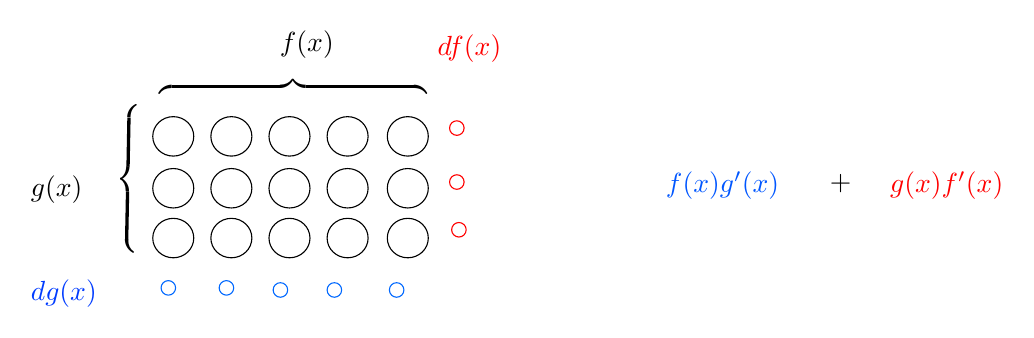
\begin{tikzpicture}[x=0.75pt,y=0.75pt,yscale=-1,xscale=1]
%uncomment if require: \path (0,300); %set diagram left start at 0, and has height of 300

%Shape: Ellipse [id:dp06031973450750061] 
\draw   (164,126.5) .. controls (164,121.25) and (168.42,117) .. (173.88,117) .. controls (179.33,117) and (183.75,121.25) .. (183.75,126.5) .. controls (183.75,131.75) and (179.33,136) .. (173.88,136) .. controls (168.42,136) and (164,131.75) .. (164,126.5) -- cycle ;
%Shape: Ellipse [id:dp8478408655553544] 
\draw   (192,126.5) .. controls (192,121.25) and (196.42,117) .. (201.88,117) .. controls (207.33,117) and (211.75,121.25) .. (211.75,126.5) .. controls (211.75,131.75) and (207.33,136) .. (201.88,136) .. controls (196.42,136) and (192,131.75) .. (192,126.5) -- cycle ;
%Shape: Ellipse [id:dp505421117341947] 
\draw   (220,126.5) .. controls (220,121.25) and (224.42,117) .. (229.88,117) .. controls (235.33,117) and (239.75,121.25) .. (239.75,126.5) .. controls (239.75,131.75) and (235.33,136) .. (229.88,136) .. controls (224.42,136) and (220,131.75) .. (220,126.5) -- cycle ;
%Shape: Ellipse [id:dp007218742660141997] 
\draw   (248,126.5) .. controls (248,121.25) and (252.42,117) .. (257.88,117) .. controls (263.33,117) and (267.75,121.25) .. (267.75,126.5) .. controls (267.75,131.75) and (263.33,136) .. (257.88,136) .. controls (252.42,136) and (248,131.75) .. (248,126.5) -- cycle ;
%Shape: Ellipse [id:dp8702465733669611] 
\draw   (277,126.5) .. controls (277,121.25) and (281.42,117) .. (286.88,117) .. controls (292.33,117) and (296.75,121.25) .. (296.75,126.5) .. controls (296.75,131.75) and (292.33,136) .. (286.88,136) .. controls (281.42,136) and (277,131.75) .. (277,126.5) -- cycle ;
%Shape: Ellipse [id:dp6716570870833466] 
\draw   (164,151.5) .. controls (164,146.25) and (168.42,142) .. (173.88,142) .. controls (179.33,142) and (183.75,146.25) .. (183.75,151.5) .. controls (183.75,156.75) and (179.33,161) .. (173.88,161) .. controls (168.42,161) and (164,156.75) .. (164,151.5) -- cycle ;
%Shape: Ellipse [id:dp1820921953890161] 
\draw   (192,151.5) .. controls (192,146.25) and (196.42,142) .. (201.88,142) .. controls (207.33,142) and (211.75,146.25) .. (211.75,151.5) .. controls (211.75,156.75) and (207.33,161) .. (201.88,161) .. controls (196.42,161) and (192,156.75) .. (192,151.5) -- cycle ;
%Shape: Ellipse [id:dp5866793827026061] 
\draw   (220,151.5) .. controls (220,146.25) and (224.42,142) .. (229.88,142) .. controls (235.33,142) and (239.75,146.25) .. (239.75,151.5) .. controls (239.75,156.75) and (235.33,161) .. (229.88,161) .. controls (224.42,161) and (220,156.75) .. (220,151.5) -- cycle ;
%Shape: Ellipse [id:dp45797332679454195] 
\draw   (248,151.5) .. controls (248,146.25) and (252.42,142) .. (257.88,142) .. controls (263.33,142) and (267.75,146.25) .. (267.75,151.5) .. controls (267.75,156.75) and (263.33,161) .. (257.88,161) .. controls (252.42,161) and (248,156.75) .. (248,151.5) -- cycle ;
%Shape: Ellipse [id:dp24430516488734677] 
\draw   (277,151.5) .. controls (277,146.25) and (281.42,142) .. (286.88,142) .. controls (292.33,142) and (296.75,146.25) .. (296.75,151.5) .. controls (296.75,156.75) and (292.33,161) .. (286.88,161) .. controls (281.42,161) and (277,156.75) .. (277,151.5) -- cycle ;
%Shape: Ellipse [id:dp5662108764983852] 
\draw   (164,175.5) .. controls (164,170.25) and (168.42,166) .. (173.88,166) .. controls (179.33,166) and (183.75,170.25) .. (183.75,175.5) .. controls (183.75,180.75) and (179.33,185) .. (173.88,185) .. controls (168.42,185) and (164,180.75) .. (164,175.5) -- cycle ;
%Shape: Ellipse [id:dp6579543801408282] 
\draw   (192,175.5) .. controls (192,170.25) and (196.42,166) .. (201.88,166) .. controls (207.33,166) and (211.75,170.25) .. (211.75,175.5) .. controls (211.75,180.75) and (207.33,185) .. (201.88,185) .. controls (196.42,185) and (192,180.75) .. (192,175.5) -- cycle ;
%Shape: Ellipse [id:dp17883475704623442] 
\draw   (220,175.5) .. controls (220,170.25) and (224.42,166) .. (229.88,166) .. controls (235.33,166) and (239.75,170.25) .. (239.75,175.5) .. controls (239.75,180.75) and (235.33,185) .. (229.88,185) .. controls (224.42,185) and (220,180.75) .. (220,175.5) -- cycle ;
%Shape: Ellipse [id:dp8959152379599131] 
\draw   (248,175.5) .. controls (248,170.25) and (252.42,166) .. (257.88,166) .. controls (263.33,166) and (267.75,170.25) .. (267.75,175.5) .. controls (267.75,180.75) and (263.33,185) .. (257.88,185) .. controls (252.42,185) and (248,180.75) .. (248,175.5) -- cycle ;
%Shape: Ellipse [id:dp8976107913184502] 
\draw   (277,175.5) .. controls (277,170.25) and (281.42,166) .. (286.88,166) .. controls (292.33,166) and (296.75,170.25) .. (296.75,175.5) .. controls (296.75,180.75) and (292.33,185) .. (286.88,185) .. controls (281.42,185) and (277,180.75) .. (277,175.5) -- cycle ;
%Shape: Circle [id:dp01856382719091243] 
\draw  [color={rgb, 255:red, 255; green, 0; blue, 0 }  ,draw opacity=1 ] (307,122.5) .. controls (307,120.57) and (308.57,119) .. (310.5,119) .. controls (312.43,119) and (314,120.57) .. (314,122.5) .. controls (314,124.43) and (312.43,126) .. (310.5,126) .. controls (308.57,126) and (307,124.43) .. (307,122.5) -- cycle ;
%Shape: Circle [id:dp4403664682847295] 
\draw  [color={rgb, 255:red, 0; green, 104; blue, 255 }  ,draw opacity=1 ] (168,199.5) .. controls (168,197.57) and (169.57,196) .. (171.5,196) .. controls (173.43,196) and (175,197.57) .. (175,199.5) .. controls (175,201.43) and (173.43,203) .. (171.5,203) .. controls (169.57,203) and (168,201.43) .. (168,199.5) -- cycle ;
%Shape: Circle [id:dp07179694909069678] 
\draw  [color={rgb, 255:red, 0; green, 104; blue, 255 }  ,draw opacity=1 ] (196,199.5) .. controls (196,197.57) and (197.57,196) .. (199.5,196) .. controls (201.43,196) and (203,197.57) .. (203,199.5) .. controls (203,201.43) and (201.43,203) .. (199.5,203) .. controls (197.57,203) and (196,201.43) .. (196,199.5) -- cycle ;
%Shape: Circle [id:dp1451673451815234] 
\draw  [color={rgb, 255:red, 0; green, 104; blue, 255 }  ,draw opacity=1 ] (222,200.5) .. controls (222,198.57) and (223.57,197) .. (225.5,197) .. controls (227.43,197) and (229,198.57) .. (229,200.5) .. controls (229,202.43) and (227.43,204) .. (225.5,204) .. controls (223.57,204) and (222,202.43) .. (222,200.5) -- cycle ;
%Shape: Circle [id:dp9161876920152885] 
\draw  [color={rgb, 255:red, 0; green, 104; blue, 255 }  ,draw opacity=1 ] (248,200.5) .. controls (248,198.57) and (249.57,197) .. (251.5,197) .. controls (253.43,197) and (255,198.57) .. (255,200.5) .. controls (255,202.43) and (253.43,204) .. (251.5,204) .. controls (249.57,204) and (248,202.43) .. (248,200.5) -- cycle ;
%Shape: Circle [id:dp7144565199430419] 
\draw  [color={rgb, 255:red, 0; green, 104; blue, 255 }  ,draw opacity=1 ] (278,200.5) .. controls (278,198.57) and (279.57,197) .. (281.5,197) .. controls (283.43,197) and (285,198.57) .. (285,200.5) .. controls (285,202.43) and (283.43,204) .. (281.5,204) .. controls (279.57,204) and (278,202.43) .. (278,200.5) -- cycle ;
%Shape: Circle [id:dp8377649456481785] 
\draw  [color={rgb, 255:red, 255; green, 0; blue, 0 }  ,draw opacity=1 ] (307,148.5) .. controls (307,146.57) and (308.57,145) .. (310.5,145) .. controls (312.43,145) and (314,146.57) .. (314,148.5) .. controls (314,150.43) and (312.43,152) .. (310.5,152) .. controls (308.57,152) and (307,150.43) .. (307,148.5) -- cycle ;
%Shape: Circle [id:dp940388133671272] 
\draw  [color={rgb, 255:red, 255; green, 0; blue, 0 }  ,draw opacity=1 ] (308,171.5) .. controls (308,169.57) and (309.57,168) .. (311.5,168) .. controls (313.43,168) and (315,169.57) .. (315,171.5) .. controls (315,173.43) and (313.43,175) .. (311.5,175) .. controls (309.57,175) and (308,173.43) .. (308,171.5) -- cycle ;

% Text Node
\draw (224,74.4) node [anchor=north west][inner sep=0.75pt]    {$f( x)$};
% Text Node
\draw (166,96.4) node [anchor=north west][inner sep=0.75pt]    {$\overbrace{\ \ \ \ \ \ \ \ \ \ \ \ \ \ \ \ \ \ \ \ \ \ \ \ \ \ \ \ \ }$};
% Text Node
\draw (145.21,183.74) node [anchor=north west][inner sep=0.75pt]  [rotate=-271.09]  {$\overbrace{\ \ \ \ \ \ \ \ \ \ \ \ \ \ \ \ }$};
% Text Node
\draw (104,144.4) node [anchor=north west][inner sep=0.75pt]    {$g( x)$};
% Text Node
\draw (300,76.4) node [anchor=north west][inner sep=0.75pt]  [color={rgb, 255:red, 255; green, 0; blue, 0 }  ,opacity=1 ]  {$df( x)$};
% Text Node
\draw (104,194.4) node [anchor=north west][inner sep=0.75pt]  [color={rgb, 255:red, 0; green, 59; blue, 255 }  ,opacity=1 ]  {$dg( x)$};
% Text Node
\draw (410,142.4) node [anchor=north west][inner sep=0.75pt]  [color={rgb, 255:red, 0; green, 86; blue, 255 }  ,opacity=1 ]  {$f( x) g'( x)$};
% Text Node
\draw (489,143.4) node [anchor=north west][inner sep=0.75pt]    {$+$};
% Text Node
\draw (518,142.4) node [anchor=north west][inner sep=0.75pt]  [color={rgb, 255:red, 255; green, 0; blue, 0 }  ,opacity=1 ]  {$g( x) f'( x)$};


\end{tikzpicture}

Basically,
\[ f \cdot g = \int f'(x)g(x) + \int g'(x)f(x) \dd x. \]
Thus, given an integral of the form of the summands, we can consider it as
\[ \int f'(x)g(x) = f(g)g(x) - \int g'(x)f(x) \dd x. \]
and
\[ \int g'(x)f(x) = f(g)g(x) - \int f'(x)g(x) \dd x. \]



\section{Applications}

\subsection{Arc length}

Take some arc we want to measure the length of.

\noindent
\begin{tikzpicture}[x=0.75pt,y=0.75pt,yscale=-1,xscale=1]
%uncomment if require: \path (0,300); %set diagram left start at 0, and has height of 300

%Shape: Axis 2D [id:dp791486377406529] 
\draw  (50,241.7) -- (314.5,241.7)(76.45,41) -- (76.45,264) (307.5,236.7) -- (314.5,241.7) -- (307.5,246.7) (71.45,48) -- (76.45,41) -- (81.45,48) (115.45,236.7) -- (115.45,246.7)(154.45,236.7) -- (154.45,246.7)(193.45,236.7) -- (193.45,246.7)(232.45,236.7) -- (232.45,246.7)(271.45,236.7) -- (271.45,246.7)(71.45,202.7) -- (81.45,202.7)(71.45,163.7) -- (81.45,163.7)(71.45,124.7) -- (81.45,124.7)(71.45,85.7) -- (81.45,85.7) ;
\draw   ;
%Curve Lines [id:da6119806462814916] 
\draw    (76.45,241.7) .. controls (112.5,67) and (290.5,90) .. (292.5,82) ;
%Shape: Axis 2D [id:dp1956952642703632] 
\draw  (370,238.7) -- (634.5,238.7)(396.45,38) -- (396.45,261) (627.5,233.7) -- (634.5,238.7) -- (627.5,243.7) (391.45,45) -- (396.45,38) -- (401.45,45) (435.45,233.7) -- (435.45,243.7)(474.45,233.7) -- (474.45,243.7)(513.45,233.7) -- (513.45,243.7)(552.45,233.7) -- (552.45,243.7)(591.45,233.7) -- (591.45,243.7)(391.45,199.7) -- (401.45,199.7)(391.45,160.7) -- (401.45,160.7)(391.45,121.7) -- (401.45,121.7)(391.45,82.7) -- (401.45,82.7) ;
\draw   ;
%Curve Lines [id:da6904688712857534] 
\draw    (396.45,238.7) .. controls (432.5,64) and (610.5,87) .. (612.5,79) ;
%Straight Lines [id:da8868203342962732] 
\draw [color={rgb, 255:red, 255; green, 0; blue, 0 }  ,draw opacity=1 ]   (396.45,238.7) -- (429.5,159) ;
%Straight Lines [id:da6732443966151707] 
\draw [color={rgb, 255:red, 255; green, 0; blue, 0 }  ,draw opacity=1 ]   (429.5,159) -- (494.5,105) ;
%Straight Lines [id:da792722354522738] 
\draw [color={rgb, 255:red, 255; green, 0; blue, 0 }  ,draw opacity=1 ]   (600.5,81) -- (494.5,105) ;
%Straight Lines [id:da7780337638207823] 
\draw [color={rgb, 255:red, 0; green, 42; blue, 255 }  ,draw opacity=1 ]   (429.5,159) -- (493.5,159) ;
%Straight Lines [id:da5469718819271276] 
\draw [color={rgb, 255:red, 0; green, 42; blue, 255 }  ,draw opacity=1 ]   (493.5,159) -- (493.5,107) ;

% Text Node
\draw (42,139.4) node [anchor=north west][inner sep=0.75pt]    {$y$};
% Text Node
\draw (174,263.4) node [anchor=north west][inner sep=0.75pt]    {$x$};
% Text Node
\draw (362,136.4) node [anchor=north west][inner sep=0.75pt]    {$y$};
% Text Node
\draw (494,260.4) node [anchor=north west][inner sep=0.75pt]    {$x$};
% Text Node
\draw (454,167.4) node [anchor=north west][inner sep=0.75pt]  [color={rgb, 255:red, 0; green, 95; blue, 255 }  ,opacity=1 ]  {$dx$};
% Text Node
\draw (504,126.4) node [anchor=north west][inner sep=0.75pt]  [color={rgb, 255:red, 0; green, 24; blue, 255 }  ,opacity=1 ]  {$dy$};
% Text Node
\draw (407,75.4) node [anchor=north west][inner sep=0.75pt]  [color={rgb, 255:red, 255; green, 0; blue, 0 }  ,opacity=1 ]  {$\sqrt{dx^{2} +dy^{2}}$};


\end{tikzpicture}

We can approximate the lengths by taking straight lines at smaller and smaller intervals.
We get the length \( \sqrt{\dd{x}^2 + \dd{y}^2} \).
Since we don't want to just add the lengths together as we take smaller \( dx \),
we can integrate instead.
But we need some rate to accumulate.
The rate we want is per \( dx \).
Thus if we take
\[ \frac{1}{dx} \sqrt{dx^2 + dy^2} = \sqrt{1 + \left(\frac{dy}{dx}\right)^2}, \]
we get the rate of accumulation of length per \( dx \),
which allows us to take the integral
\[ \sqrt{1 + \left(\frac{dy}{dx}\right)^2} \dd x \]
to get the total length.

\end{document}